% move results for Beatles and Witnesses to beginning of section 6, rename section, say a bit more about these results, make sure desiderata are clear in the subsections introducing the scenarios



%polaczyc tableki sally clark, SC 





\documentclass[10pt,]{scrartcl}
 \usepackage{lmodern}
\usepackage{amssymb,amsmath}
\usepackage{ifxetex,ifluatex}
\usepackage{fixltx2e} % provides \textsubscript
\ifnum 0\ifxetex 1\fi\ifluatex 1\fi=0 % if pdftex
  \usepackage[T1]{fontenc}
  \usepackage[utf8]{inputenc}
\else % if luatex or xelatex
  \ifxetex
    \usepackage{mathspec}
  \else
    \usepackage{fontspec}
  \fi
  \defaultfontfeatures{Ligatures=TeX,Scale=MatchLowercase}
\fi
% use upquote if available, for straight quotes in verbatim environments
\IfFileExists{upquote.sty}{\usepackage{upquote}}{}
% use microtype if available
\IfFileExists{microtype.sty}{%
\usepackage[]{microtype}
\UseMicrotypeSet[protrusion]{basicmath} % disable protrusion for tt fonts
}{}
\PassOptionsToPackage{hyphens}{url} % url is loaded by hyperref
\usepackage[unicode=true]{hyperref}
\PassOptionsToPackage{usenames,dvipsnames}{color} % color is loaded by hyperref
\hypersetup{
            pdftitle={Measuring coherence with Bayesian Networks},
            colorlinks=true,
            linkcolor=blue,
            citecolor=blue,
            urlcolor=blue,
            breaklinks=true}
\urlstyle{same}  % don't use monospace font for urls
\usepackage{graphicx,grffile}
\makeatletter
\def\maxwidth{\ifdim\Gin@nat@width>\linewidth\linewidth\else\Gin@nat@width\fi}
\def\maxheight{\ifdim\Gin@nat@height>\textheight\textheight\else\Gin@nat@height\fi}
\makeatother
% Scale images if necessary, so that they will not overflow the page
% margins by default, and it is still possible to overwrite the defaults
% using explicit options in \includegraphics[width, height, ...]{}
\setkeys{Gin}{width=\maxwidth,height=\maxheight,keepaspectratio}
\IfFileExists{parskip.sty}{%
\usepackage{parskip}
}{% else
\setlength{\parindent}{0pt}
\setlength{\parskip}{6pt plus 2pt minus 1pt}
}
\setlength{\emergencystretch}{3em}  % prevent overfull lines
\providecommand{\tightlist}{%
  \setlength{\itemsep}{0pt}\setlength{\parskip}{0pt}}
\setcounter{secnumdepth}{5}
% Redefines (sub)paragraphs to behave more like sections
\ifx\paragraph\undefined\else
\let\oldparagraph\paragraph
\renewcommand{\paragraph}[1]{\oldparagraph{#1}\mbox{}}
\fi
\ifx\subparagraph\undefined\else
\let\oldsubparagraph\subparagraph
\renewcommand{\subparagraph}[1]{\oldsubparagraph{#1}\mbox{}}
\fi

% set default figure placement to htbp
\makeatletter
\def\fps@figure{htbp}
\makeatother

%\documentclass{article}

\usepackage[table]{xcolor
}


% %packages
 \usepackage{booktabs}
 \usepackage[sort&compress]{natbib}
\usepackage{graphicx}
\usepackage{longtable}
\usepackage{ragged2e}
\usepackage{etex}
%\usepackage{yfonts}
\usepackage{marvosym}
\usepackage[notextcomp]{kpfonts}
\usepackage{nicefrac}
\newcommand*{\QED}{\hfill \footnotesize {\sc Q.e.d.}}

\usepackage[textsize=footnotesize]{todonotes}
%\linespread{1.5}



\setlength{\parindent}{10pt}
\setlength{\parskip}{1pt}


%language
%\usepackage{times}
\usepackage{mathptmx}
\usepackage{t1enc}
%\usepackage[utf8x]{inputenc}
%\usepackage[polish]{babel}
%\usepackage{polski}

\usepackage{subcaption}


%AMS
\usepackage{amsfonts}
\usepackage{amssymb}
\usepackage{amsthm}
\usepackage{amsmath}

%\usepackage{geometry}
 %\geometry{a4paper,left=35mm,top=20mm,}

%abbreviations
\newcommand{\ra}{\rangle}
\newcommand{\la}{\langle}
\newcommand{\n}{\neg}
\newcommand{\et}{\wedge}
\newcommand{\jt}{\rightarrow}
\newcommand{\ko}[1]{\forall  #1\,}
\newcommand{\ro}{\leftrightarrow}
\newcommand{\exi}[1]{\exists\, {_{#1}}}
\newcommand{\pr}{\mathsf{P}}
\newcommand{\odds}{\mathsf{Odds}}
\newcommand{\ind}{\mathsf{Ind}}
\newcommand{\nf}[2]{\nicefrac{#1\,}{#2}}
\newcommand{\R}[1]{\texttt{#1}}

\newtheorem{q}{\color{blue}Question}



\newcommand{\s}[1]{\mbox{\textsf{#1}}}



\newtheorem*{reply*}{Reply}
\usepackage{enumitem}
\newcommand{\question}[1]{\begin{enumerate}[resume,leftmargin=0cm,labelsep=0cm,align=left]
\item #1
\end{enumerate}}

\usepackage{float}
 
\title{Measuring coherence with Bayesian Networks}
\author{}
\date{\vspace{-2.5em}}

\begin{document}
\maketitle
\tableofcontents

\section{Motivations \& introduction}


When we talk about the coherence of a set of propositions or about the
coherence of a story, we seem to refer to how well their individual
pieces fit together. How are we to understand and apply this notion
systematically, though?  As with beliefs, we can use both a binary and a graded notion of coherence. The binary notion is not very exciting: a set is incoherent
just in case it is logically
inconsistent.\footnote{There is a related notion in the neighborhood where an agent's  degrees of beliefs are coherent just in case it they are probabilistic. We will not use this notion in this paper.}  Our basic intuition is that graded coherence should satisfy  a generalization of this requirement: logically incoherent sets should have minimal level of graded coherence or, at least, lower coherence than consistent ones.  The goal of the paper is to provide an explication of the notion of coherence    that satisfies this requirement and  performs better than other measures. The key improvement  is that  once a narration is represented as a Bayesian network, its coherence is determined not only by the underlying probability measure, but also by the network structure. 



Why do we need an explication of the notion of coherence, though? 
First, it is philosophically desirable, as  the notion is often used in many philosophical, especially
epistemological, discussions \citep[for instance, in discussions about the truth-conduciveness of coherence,][]{shogenji1999conducive,olsson2001conducive}.  Second, a  plausible measure of coherence could be used to better evaluate the quality of  stories or narrations. One example  when it would be useful, is in the assessment of the quality of  narations in the court of law. Focusing only on the probability of a story is to some extent problematic, because from such a perspective, more detailed stories are penalized---they contain more propositions, so they (usually) have lower probabilities.  






Interestingly, there is a disconnect between philosophical research on probabilistic coherence and the development of  Bayesian networks--based methods. The latter seems  unaware of the philosophical discussion, and the philosophical discussions of coherence do not refer to  Bayesian networks. Our paper  narrows this gap.



In a  Bayesian networks approach to  modeling stories and narrations in legal contexts.
\citet{vlek2013modeling} proposed an account  on which the coherence of a story (represented by a whole Bayesian network)
is captured by the addition of a single narration root node.\footnote{The root node  becomes an ancestor
node to all the other nodes such that the conditional probability of
each dependent node given that the state of this root is 1 (that is, the
corresponding proposition is assumed to be true), is also 1. See \citep{vlek2014building,vlek2015,vlek2016method,vlek2016stories} for more details, and \citep{fenton2013general} for another take on Bayesian network representation of narrations.}  Its prior probability is identified with coherence. We think this approach is too simplistic, as we want to capture the idea that coherence is distinct
from probability, and  the addition of a scenario node  introduces probabilistic
dependencies by fiat. 










% to asses an important aspect of a narration which
%so far seems to escape probabilistic analysis.





Our measure diverges from the known candidates in three important
respects: (1) It is not a function of a probability measure and a set
of propositions alone, because it is also sensitive to the selection and
direction of arrows in a Bayesian Network representing an agent's credal state. (2) Unlike in the case of quite a few coherence measures, it is  sensitive to
 the  weakest links in the narration.
(3) It is not obtained by simply averaging confirmation levels between all possible combinations of elements.



We first describe the main probabilistic explications of coherence present in the literature (Section \ref{sec:measures}). Then, we describe two philosophically motivated thought experiments and one real-life example that will serve as illustration in our Bayesian network approach (Section \ref{sec:senariosAndBns}). Next we try to identify the key problems with  the existing measures (Section \ref{sec:challenges}), which leads us to our own positive proposal---that of \emph{structured coherence} (Section \ref{sec:structured}), which we explain with a running example in the background. With this tool in hand we approach our real-life example (the Sally Clark case) and argue that our measure handles it better than the other measures (Section \ref{sec:Sally}). We finish with the comparison of our measure with respect to the other examples we used, and a few closing comments (Section \ref{sec:discussion}). 





\section{Measures}\label{sec:measures}

Quite a few different measures of coherence have already been developed.  Two early proposals are the so-called deviation from independence measure and  the relative overlap measure.

\begin{itemize}
    \item  Shogenji's 
  \textit{deviation from independence} \citep{shogenji1999conducive}, is defined as the ratio between the probability of the
conjunction of all claims, and the probability that the conjunction
would get if all its conjuncts were probabilistically independent (scaling from 0 to $\infty$ with neutral point 1):

\begin{align}
    \tag{Shogenji}
    \label{coh:Shogenji}
     \mathcal{C}_{S}(S)=\frac{P(\bigwedge S)}{\prod_{i=1}^{\vert S \vert}\{P(S_i)\vert i \in S\}}
\end{align}

\item  \textit{Relative overlap} coming from \citep{olsson2001conducive} and \citep{glass2002}, is defined as the ratio  between the intersection of all propositions and their union (scaling from -1 to 1 with no clear neutral point):

\begin{align}
    \tag{Olsson}
    \label{coh:Olsson}
    \mathcal{C}_{O}(S)=\frac{P(\bigwedge S)}{P(\bigvee S)}
\end{align}


\end{itemize}

Both of these approaches are susceptible to various objections and counterexamples \citep{Merricks1995,shogenji1999conducive, Akiba2000Shogenjis, Shogenji2001Reply, bovens2004bayesian,Siebel2004On-Fitelsons-me,siebel2006against,Shogenji2006Why,crupi2007BayesianMeasuresEvidential, koscholke2016evaluating, Schippers2019General}, To overcome them, more  recent works developed  a class of measures called
\textit{average mutual support}. Let’s take a look at  the general recipe for such a measure.


\begin{itemize}
\item
  Given that \(S\) is a set whose coherence is to be measured, let \(P\)
  indicate the set of all ordered pairs of non-empty, disjoint subsets
  of \(S\).
\item
  First, define a confirmation measure for the confirmation of a hypothesis \(H\) by evidence  \(E\): \(Conf(H,E)\).
\item
  For each pair \(\langle X, Y \rangle \in P\), calculate
  \(Conf(\bigwedge X, \bigwedge Y)\), where $\bigwedge X$  is the conjunction of all the elements of $X$ (and $\bigwedge Y$ is to be understood analogously).
\item
  Take the mean of all the results.
\end{itemize}\begin{align*}
    \mathcal{C}(S) & =
mean\left(\left\{Conf(\bigwedge X_i, \bigwedge Y_i) | \langle X_i, Y_i \rangle \in P\right\} \right)
\end{align*}

\noindent Depending on the choice of a confirmation measure, we achieve
different measures of coherence.  One thing to keep in mind is
that different measures use different scales and have different neutral points, if any (the idea is: the coherence of probabilistically independent propositions should be neither positive nor
negative). Here are the key candidates present in the literature:

\begin{itemize}

\item \citet{fitelson2003ProbabilisticTheoryCoherence}   uses the following confirmation function (the resulting coherence measure ranges from -1 to 1 with neutral point at 0):

\begin{align*}
    F(H,E) = \begin{cases}
    1 & E\models H, E\not \models \bot \\
    -1 & E \models \neg H\\
    \frac{P(E|H)-P(E|\neg H)}{P(E|H)+P(E|\neg H)} & \mbox{o/w}
    \end{cases}
\end{align*}
\begin{align}
\tag{Fitelson}  
    \mathcal{C}_{F}(S) & =
mean\left(\left\{F(\bigwedge X_i, \bigwedge Y_i) | \langle X_i, Y_i\rangle \in P\right\} \right)
\end{align}

%\noindent For instance, Fitelson's coherence for two propositions boils
%down to this:

%\begin{align}    
%    \tag{Fitelson pairs}  
%    \mathcal{C}_{F}(X,Y) &= %    \label{coh:Fitelson}
%\end{align}

%\noindent \textbf{scale:} {[}-1, 1{]}

%\noindent \textbf{neutral point:} 0

%\subsection{Douven and Meij's}

\item  \citet{Douven2007measuring}  use the \textit{difference} confirmation measure (with coherence ranging from -1 to 1 with neutral point at 0):

\begin{align*}
    D(H,E) = P(H|E) - P(H)
\end{align*}
\begin{align}
\tag{DM}  
    \mathcal{C}_{DM}(S) & =
mean\left(\left\{D(\bigwedge X_i, \bigwedge Y_i) | \langle X_i, Y_i\rangle \in P\right\} \right)
\end{align}

%For two propositions, the coherence measure boils down to:

%\begin{align}
%    \tag{DM pairs}
%    \label{coh:DM}
%    C_{DM}(X,Y)= \frac{P(X|Y) - P(X) + P(Y|X) - P(Y)}{2}
%\end{align}

%\noindent \textbf{scale:} {[}-1, 1{]}

%\noindent \textbf{neutral point:} 0 (not explicit)

\item  \citet{Roche2013Coherence} uses the
absolute confirmation measure (the resulting coherence measure ranges from 0 to 1 with neutral point at $0.5$): 

\begin{align*}
    A(H,E) = \begin{cases}
    1 & E\models H, E\not \models \bot \\
    0 & E \models \neg H\\
    P(H|E) & \mbox{o/w} \\
    \end{cases}
\end{align*}
\begin{align}
\tag{Roche}  
    \mathcal{C}_{R}(S) & =
mean\left(\left\{A(\bigwedge X_i, \bigwedge Y_i) | \langle X_i, Y_i\rangle \in P\right\} \right) 
\end{align}

%For two propositions, the measure gives the following:

%\begin{align}
%    \tag{Roche pairs}
%    \label{coh:Roche}
%     C_{R}(X,Y)= \frac{P(X|Y)+P(Y|X)}{2}
%\end{align}

\end{itemize}











\section{Scenarios and Bayesian Networks}\label{sec:senariosAndBns}


One important way to evaluate coherence measures is to look at how they behave in test scenarios.\footnote{Another way present in the literature is to formulate abstract formal requirements for a coherence measure and to investigate whether a given coherence measure satisfies them. Since there is no agreement in the literature on what such requirements should be, we decided not to take this path in this paper.}
 Some of those come from philosophical literature, and were put forward as counterexamples: they usually have the form of a few propositions formulated in natural language, such that intuitive judgments of coherence involved and the formal coherence calculations  diverge.  Due to space limitations we will only bring up a couple of them to illustrate what we think the key problems with the existing measures are. We are aware of other cases (Penguins \citep{bovens2004bayesian,Meijs2007Alleged},  Dunnit \citep{Merricks1995}, 
Japanese swords \citep{Meijs2007Alleged}, 
Robbers \citep{Siebel2004On-Fitelsons-me},
and two similar ones: Depth and 
Dice  \citep{Akiba2000Shogenjis,Shogenji2001Reply,Schippers2019General}), but their  treatment is postponed to a different paper.

More importantly, we will also include a real-life example of the famous Sally Clark case. As we intend our measure to have practical applications, we need a sanity check of taking a look at how it behaves in a real-life scenario. 

 In this section we introduce the scenarios we will use, describe how we capture them using Bayesian networks, and mention coherence-related intuitions that seem to accompany them. 







\subsection{The Beatles}

 The Beatles example has been offered by \citet[339]{shogenji1999conducive} to criticize defining coherence of a set in terms of 
coherence of pairwise coherence.   The scenario consists of the following claims:

\begin{table}[H]
\centering
\begin{tabular}{ll}
\toprule
node & content\\
\midrule
\cellcolor{gray!6}{D} & \cellcolor{gray!6}{Exactly one of the Beatles (John, Paul, George and Ringo) is dead.}\\
J & John is alive.\\
\cellcolor{gray!6}{P} & \cellcolor{gray!6}{Paul is alive.}\\
G & George is alive.\\
\cellcolor{gray!6}{R} & \cellcolor{gray!6}{Ringo is alive.}\\
\bottomrule
\end{tabular}
\caption{Nodes in the Beatles scenario.}
\label{tab:beatles}
\end{table}

The key observation here is that each proper subset of the set is consistent, the whole set is not. So the coherence of the whole set should be lower than the coherence of each proper subset thereof.

In our representation of the scenario by means of a Bayesian network,  we assume the prior probability of each individual band member being
dead to be 0.5 (as in the above table), and the conditional probability table (CPT) for node \textsf{D} is
many-dimensional and so difficult to present concisely, but the method
is straightforward: probability 1 is given to node \textsf{D} in all
combinations of the parents in which exactly one is false, and otherwise
\textsf{D} gets conditional probability 0. The BN with marginal probabilities looks as in Figure \ref{fig:BeatlesBN3}.





\begin{figure}[H]
\centering
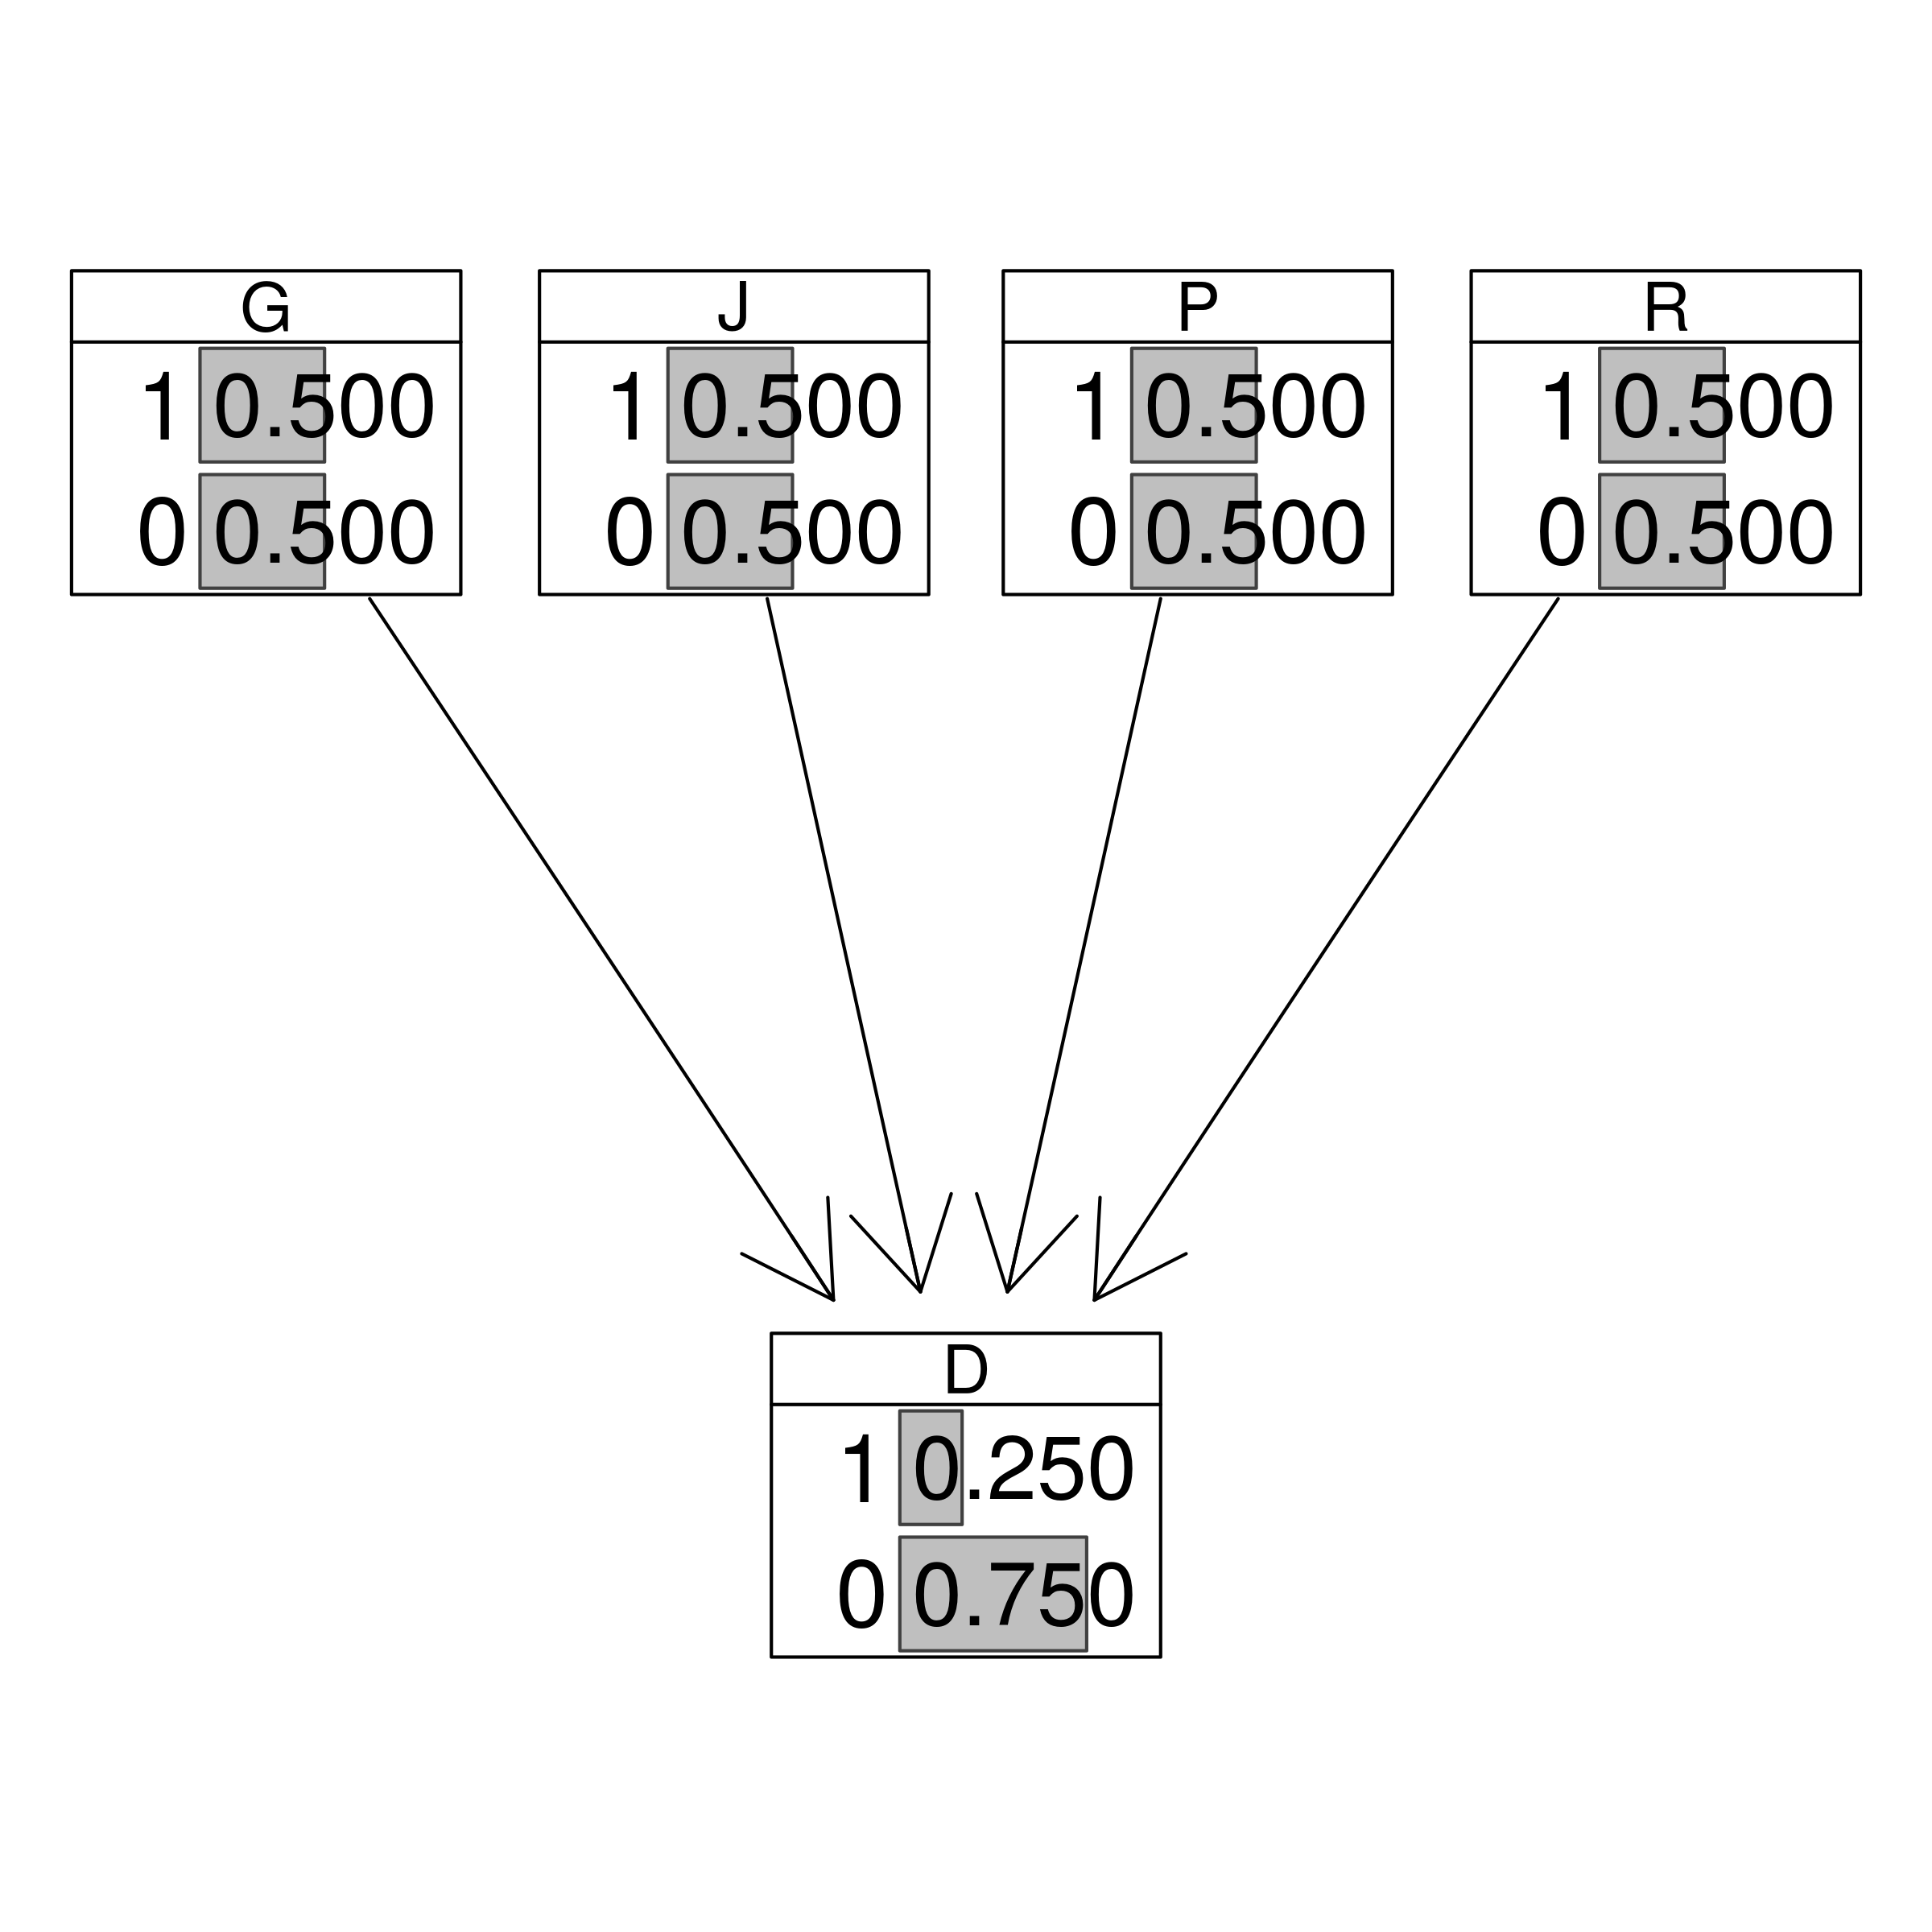
\includegraphics[width =10cm]{../images/BeatlesBN.png}
\caption{Beatles BN with marginal probabilities.}
\label{fig:BeatlesBN3}
\end{figure}




\subsection{The Witnesses}

The witnesses scenario  comes from \citep[391]{olsson2005}. Equally reliable witnesses try to identify a criminal. Consider the
 potential reports (we extended the original scenario by adding \s{W5}) listed in Table \ref{tab:witRep}. 

\begin{table}[H]
\centering
\begin{tabular}{ll}
\toprule
node & content\\
\midrule
\cellcolor{gray!6}{W1} & \cellcolor{gray!6}{Witness no. 1: ‘‘Steve did it’’}\\
W2 & Witness no. 2: ‘‘Steve did it’’\\
\cellcolor{gray!6}{W3} & \cellcolor{gray!6}{Witness no. 3: ‘‘Steve, Martin or David did it’’}\\
W4 & Witness no. 4: ‘‘Steve, John or James did it’’\\
\cellcolor{gray!6}{W5} & \cellcolor{gray!6}{Wittness no. 5: ‘‘Steve, John or Peter did it’’}\\
D & Who committed the deed (6  possible values)\\
\bottomrule
\end{tabular}
\caption{Potential witness reports in the witness scenario.}
\label{tab:witRep}
\end{table}

\noindent Note that  each proposition has the structure ``Witness no.
\(X\) claims that \dots" instead of explicitly stating the witness'
testimony.

Two requirements are associated with this example: both
\(\{\)\textsf{W1, W2}\(\}\) and \(\{\)\textsf{W4, W5}\(\}\) should be
more coherent than \(\{\)\textsf{W3, W4}\(\}\).  The underlying intuition is the more suspects the witnesses agree on, the more coherent the evidence. 


In our BN representation, each of these three sets is represented by a network with three nodes: the root note \textsf{D} (who actually committed the deed), and its two binary children nodes corresponding to the propositions contained in a given set. Figure \ref{fig:witnessw1w2} illustrates the DAG for the first set, together with the marginal probabilities. The other two networks are analogous.


The basic idea behind
the CPTs we used is that for any particular witness we take the
probability of them including the perpetrator in their list to be 0.8,
and the probability of including an innocent to be .05.  
The CPT for \textsf{D} is uniform. The table for \textsf{W1}  (Table \ref{tab:w1w2}) provides
the conditional probability of \textsf{W1} listing (\textsf{W1}=1) or
not listing (\textsf{W1}=0) a particular person given that the actual
value of \textsf{D} is Steve/Martin/\dots.  In the
Bayesian networks for other witness scenarios,  the CPT for \textsf{D} remains the same, and the CPTs for the witness nodes are analogous to the one for \textsf{W1}. 






\begin{figure}[h]
\centering
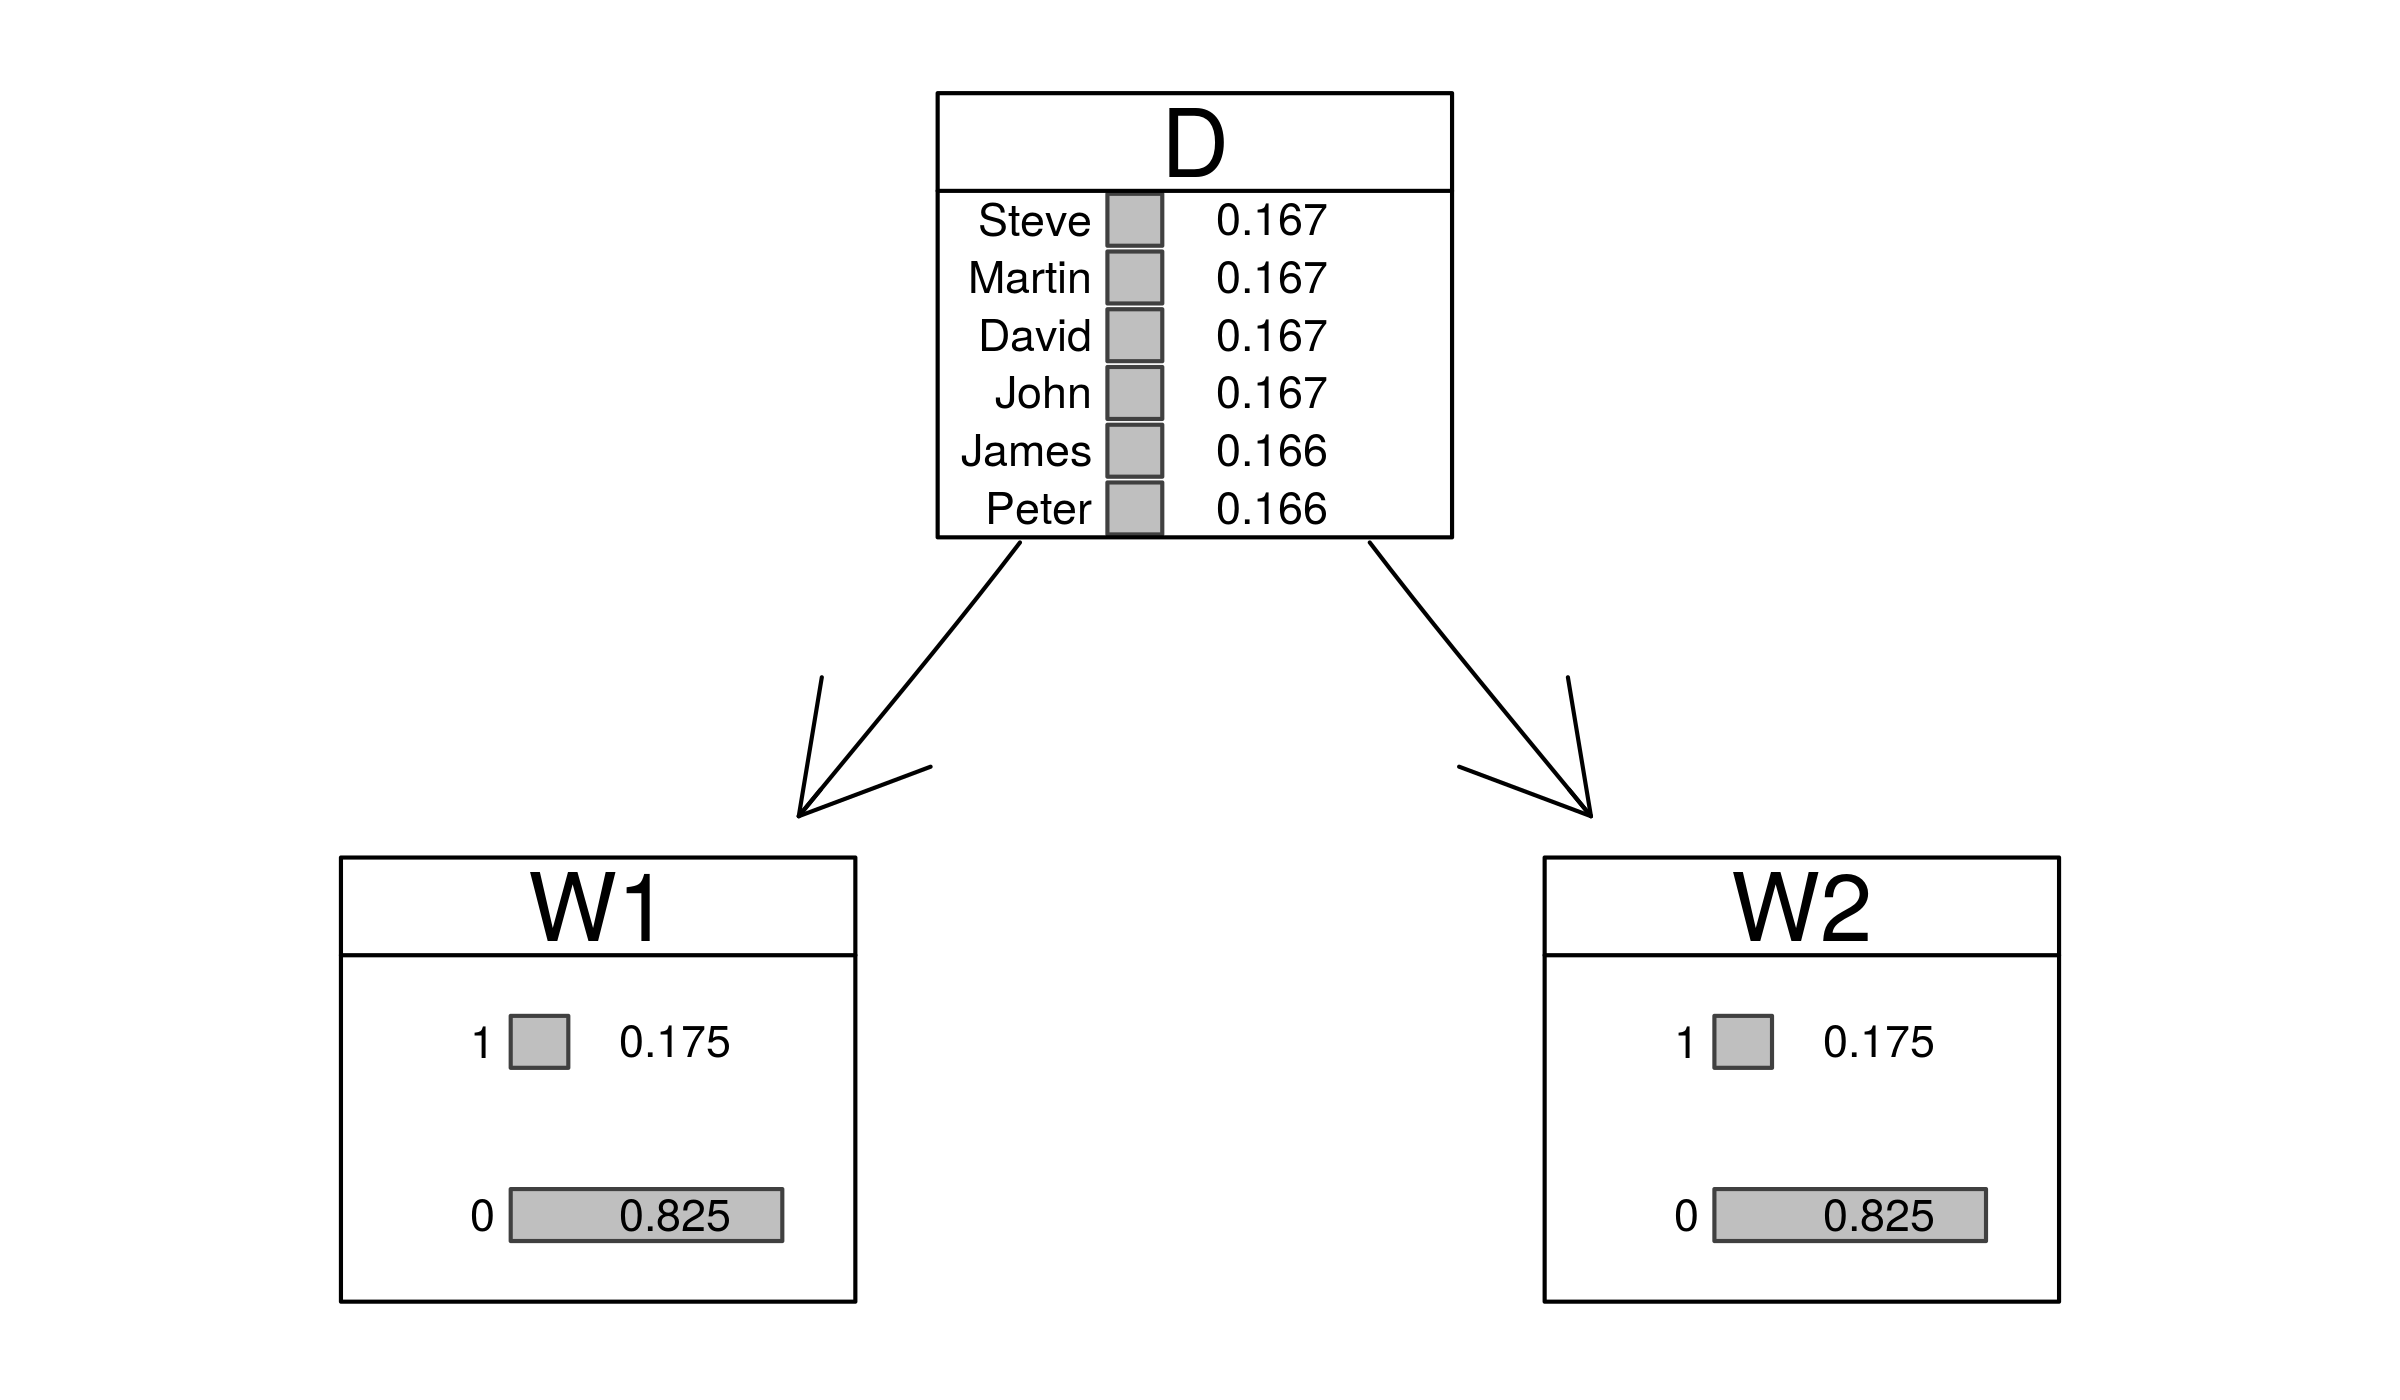
\includegraphics[width =14cm]{../images/w1w2BNv2.png}
\caption{BN for the witnesses example (W1W2) with marginal probabilities.}
\label{fig:witnessw1w2}
\end{figure}







%\begin{figure}

%\hspace{-15mm} 
%\begin{subfigure}[!ht]{0.3\textwidth}
\begin{table}[H]
% \centering
% \begin{tabular}{lr}
% \toprule
% D & Pr\\
% \midrule
% \cellcolor{gray!6}{Steve} & \cellcolor{gray!6}{0.167}\\
% Martin & 0.167\\
% \cellcolor{gray!6}{David} & \cellcolor{gray!6}{0.167}\\
% John & 0.167\\
% \cellcolor{gray!6}{James} & \cellcolor{gray!6}{0.167}\\
% Peter & 0.167\\
% \bottomrule
% \end{tabular}
% \end{table}
% \end{subfigure}
% \begin{subfigure}[!ht]{0.2\textwidth}
\centering
\begin{tabular}{lrrrrrr}
\toprule
\multicolumn{1}{c}{W1} & \multicolumn{2}{c}{D} \\
  & Steve & Martin & David & John & James & Peter\\
\midrule
\cellcolor{gray!6}{\cellcolor{gray!6}{1}} & \cellcolor{gray!6}{\cellcolor{gray!6}{0.8}} & \cellcolor{gray!6}{\cellcolor{gray!6}{0.05}} & \cellcolor{gray!6}{\cellcolor{gray!6}{0.05}} & \cellcolor{gray!6}{\cellcolor{gray!6}{0.05}} & \cellcolor{gray!6}{\cellcolor{gray!6}{0.05}} & \cellcolor{gray!6}{\cellcolor{gray!6}{0.05}}\\
0 & 0.2 & 0.95 & 0.95 & 0.95 & 0.95 & 0.95\\
\bottomrule
\end{tabular}
% \end{table}
% \end{subfigure}
\caption{CPT for \textsf{W1} in the \textsf{W1W2} scenario. CPTs for other witnesses are  analogous.}
\label{tab:w1w2}
\end{table}


%This is our baseline BN for the scenario. In our measure, however, we will use as weights the probabilities that result from updating the BN with the scenario, as the coherence of a scenario is to be evaluated from its own perspective (we'll have a bit more say about this later on). 







% \textbf{Desiderata.} First, we can observe that \s{W1} and \s{W2} fully
% agree. Testimonies of \s{W3} and \s{W4} overlap only partially,
% therefore it seems that \{\s{W1},\s{W2}\} is more coherent than
% \{\s{W3},\s{W4}\}. \vspace{2mm}

% \begin{description}
%     \item[(\s{W1W2\textgreater W3W4})] \{\s{W1},\s{W2}\} should be more coherent than \{\s{W3},\s{W4}\}.
% \end{description}

% \vspace{2mm}

% Similarly, there is a greater agreement between \s{W4} and \s{W5} than
% \s{W3} and \s{W4}, so \{\s{W4},\s{W5}\} seems more coherent than
% \{\s{W3},\s{W4}\}. \vspace{2mm}

% \begin{description}
%     \item[(\s{W4W5\textgreater W3W4})] \{\s{W4},\s{W5}\} should be more coherent than \{\s{W3},\s{W4}\}.
% \end{description}

% \vspace{2mm}





\subsection{Sally Clark}



Later on we take the existing coherence measures for a ride by testing them on a real-case based Bayesian network for the Sally Clark case. At this point, we introduce the case and the network.  

R. v. Clark (EWCA Crim 54, 2000) is a classic  example of how the lack of probabilistic independence between events can be easily overlooked. Sally Clark's first son died in 1996 soon after birth, and her second son died in similar circumstances a few years later in 1998.  At trial, the paediatrician Roy Meadow testified that the probability that a child from such a  family would die of Sudden Infant Death Syndrome (SIDS) was 1 in 8,543.  Meadow calculated that therefore the probability of both children dying of SIDS was approximately  1 in 73 million. Sally Clark was convicted of murdering her  infant sons (the conviction was ultimately reversed on appeal). The calculation illegitimately assumes independence,  as the  environmental or genetic factors may predispose a family to SIDS. The winning appeal was based on new evidence: signs of a potentially lethal disease---contrary to what was assumed in the original case---were found in one of the bodies. 

We will be interested in tracking probability and coherence in three stages of the case: 
\begin{itemize} 
\item In \textsf{Stage 0}, it is known that the children have died, but no evidence regarding bruising or traces of disease is available.

\item In \textsf{Stage 1}, which corresponds to the original case, bruising is found in two children, but no trace of disease in either.

\item In \textsf{Stage 2}, bruising was found in both sons, but signs of disease are also present in the first son. 
\end{itemize}



Here  are some intuitions one might have about the coherences involved. Let's call the scenario in which both children died of SIDS 00, the one in which both were murdered 11, the one in which only the first child was murdered 10, and the one in which only the second one was murdered 01.

\begin{enumerate}
    \item We would expect 11 and 00 to be more coherent than either 10 or 01. The intution is that the claim that both sons died in the same way sounds more coherent than the alternative scenarios.  %This condition is satisfied by all measures.
    %This requirement fails for Douven-Meijs and Shogenji.
    \item Perhaps, we would not expect 11 and 00 to be nearly maximally coherent. If we buy into this intuiton, we have reasons to dislike Fitelson, Roche and Olsson-Glass.
    \item When moving from Stage 0 to Stage 1, the coherence of 11 should not decrease. After all, we include evidence in support of 11. This condition fails for Douven-Meijs, Shogenji and to a slight extent for Fitelson.
    \item For similar reason, we would not expect the coherence of 11 to be much less than the coherence of 00 in Stage A. This condition fails for Douven-Meijs and Shogenji.
    \item Given that in Stage B we include evidence supporting the claim that son A was not murdered, we would not expect the coherence of 01 to be smaller than the coherence of 10 in Stage B. This condition fails radically for Fitelson (01 becomes maximally incoherent, even though the evidence is not conclusive!), and to a small degree for Douven-Meijs.

    \item  One might have the intuition that \textsf{Stage 0}expect the coherences of 11 and 00 to not be too far. While perhaps 00 should have lower prior probability than 11,  prior to obtaining evidence, mere coherence considerations don't seem to put one of these scenarios at a strong disadvantage.
\end{enumerate}












\citet{Fenton2018Risk} constructed a Bayesian network to discuss the interaction of the key pieces of evidence in this case, and our Bayesian network is based on theirs.  The network structure is in Figure \ref{fig:sc}.


\begin{figure}[H]
    \centering
    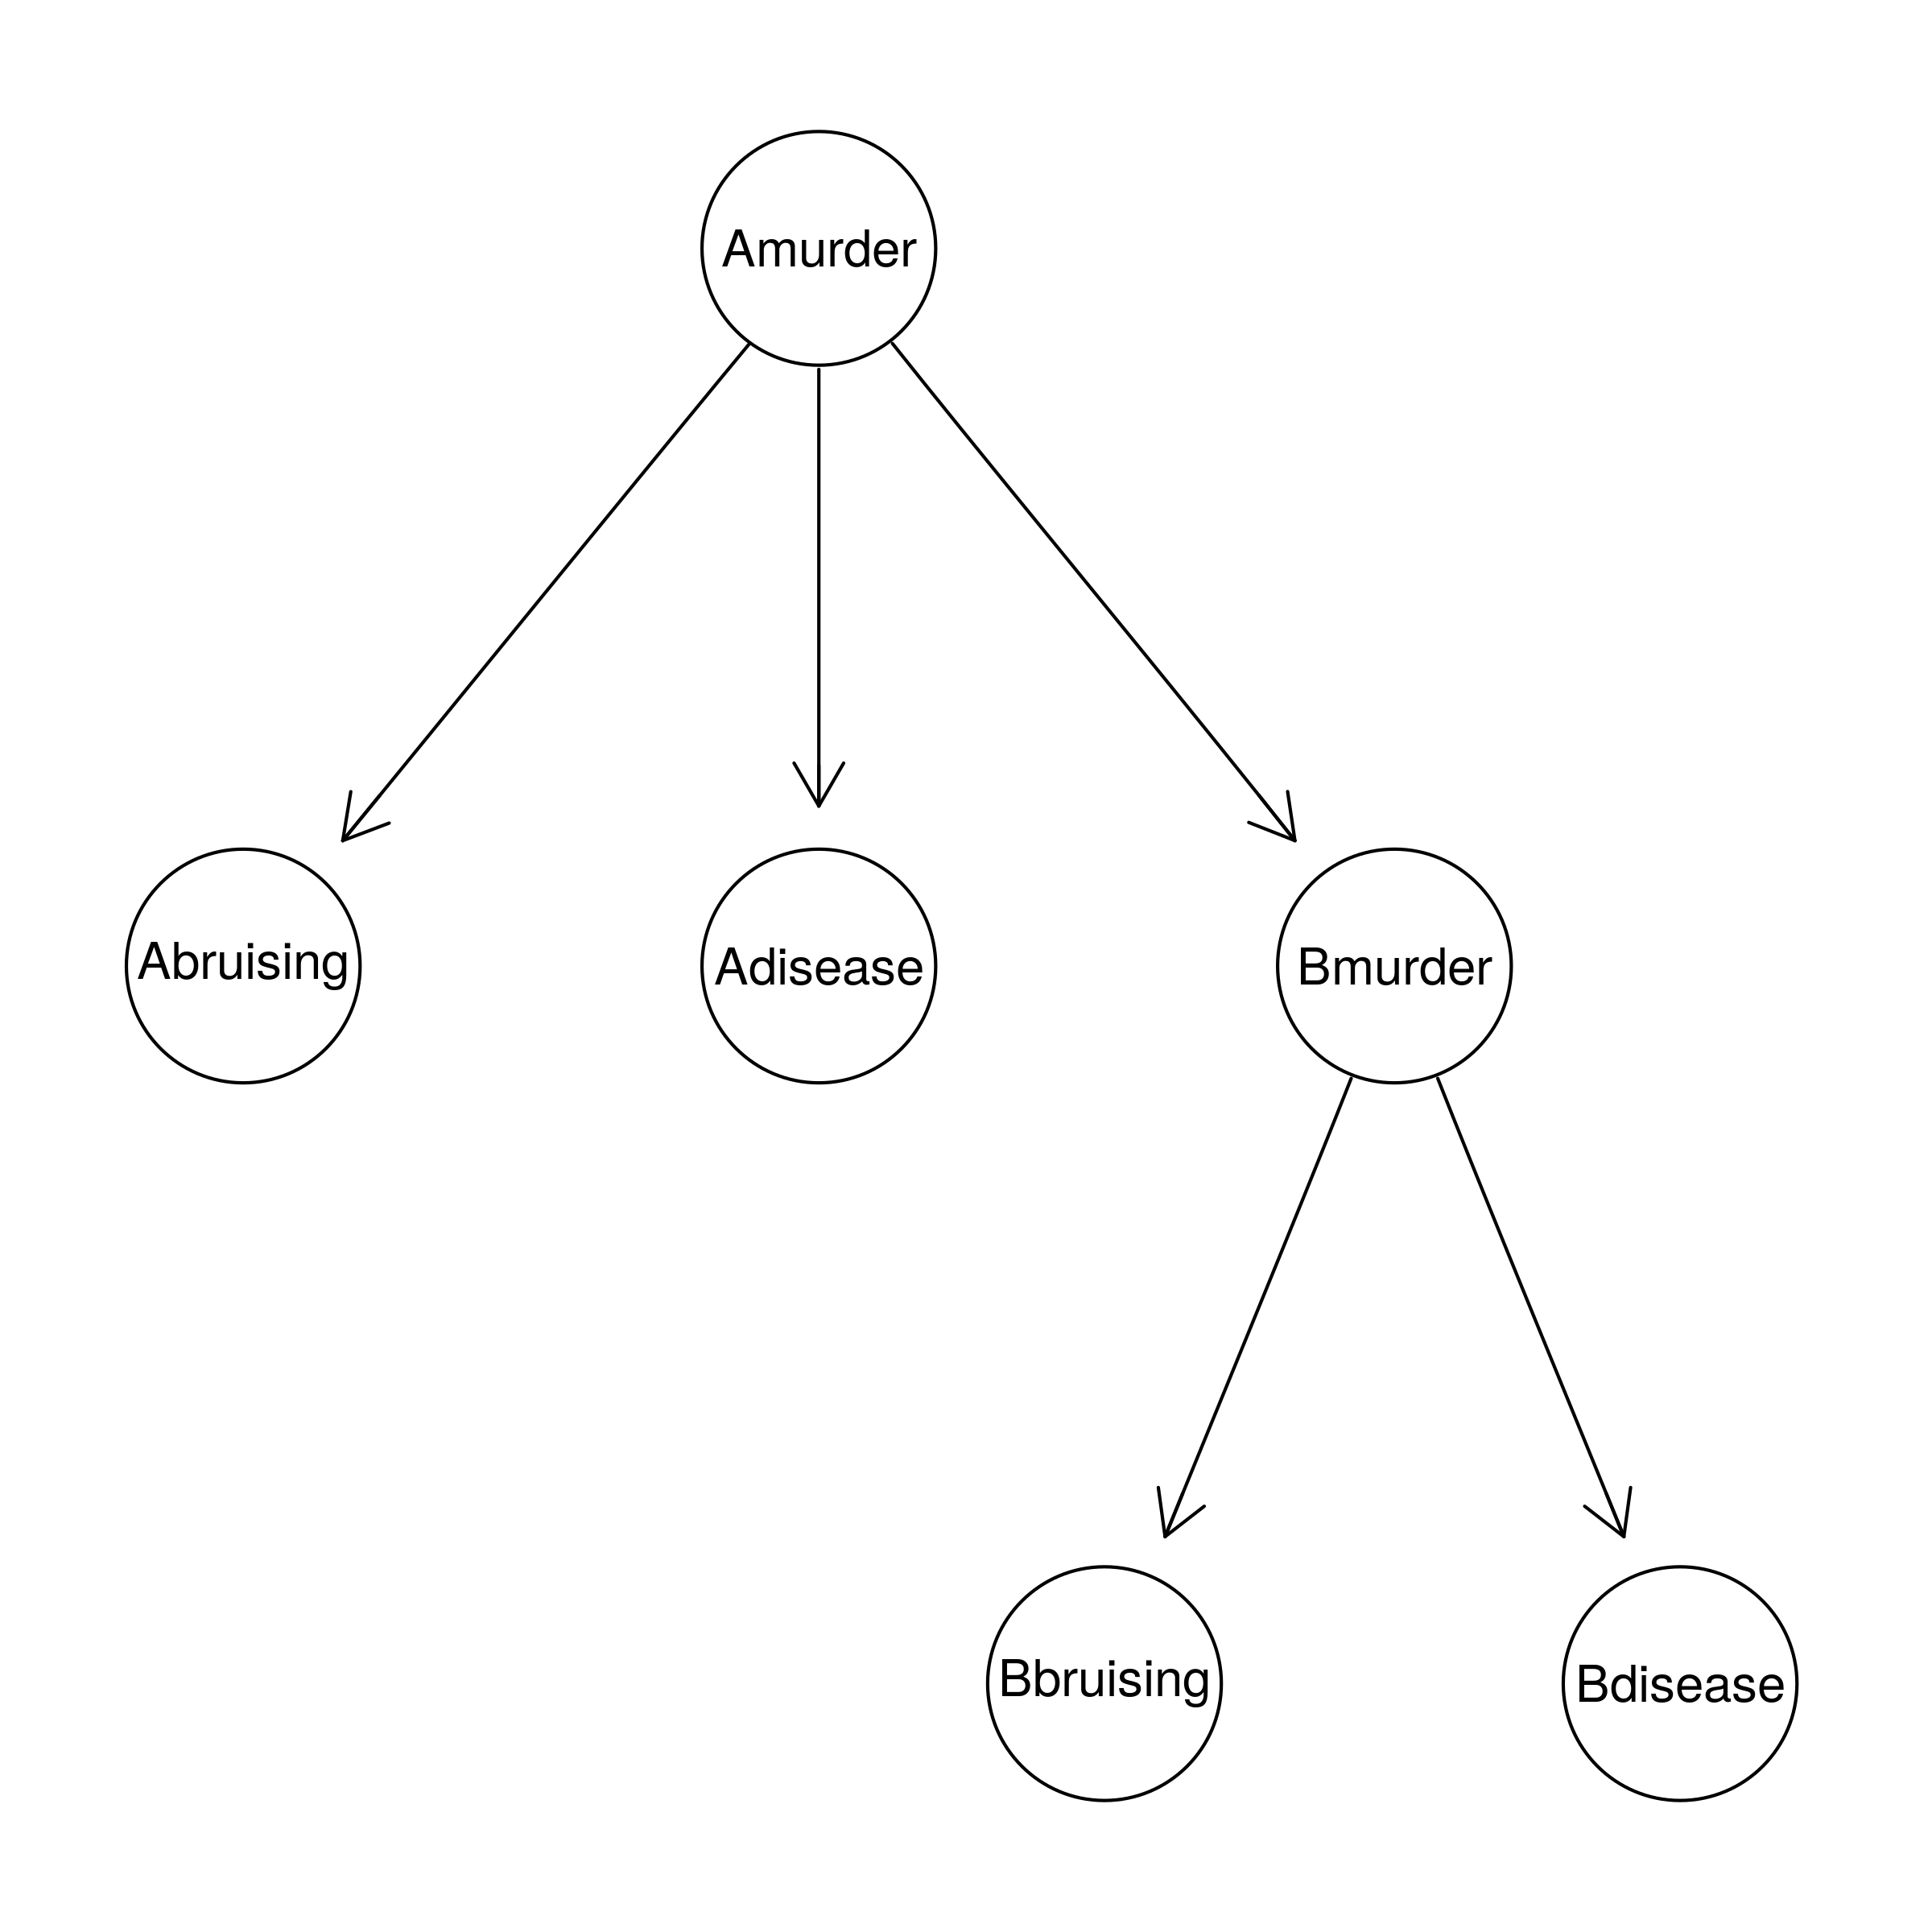
\includegraphics[width = 12cm]{SC.png}
    \caption{The directed acyclic graph for the Sally Clark BN}
    \label{fig:sc}
\end{figure}



The  arrows  depict  relationships  of  influence  between  variables. \textsf{Amurder} and \textsf{Bmurder} are binary nodes corresponding to whether Sally  Clark’s  sons,   call  them A and B, were murdered. These  influence  whether  signs of disease (\textsf{Adisease} and \textsf{Bdisease}) and bruising (\textsf{Abruising} and \textsf{B.bruising}) were present. Also, since  son A died first, whether A was murdered casts some light on the probability of son B being murdered.

We employ the same probability tables as \citet{Fenton2018Risk}, which incorporated Mr Meadow's statistical testimony. The prior probability of son A not being murdered is $0.921659$, the probability of bruising in a son if he wasn't murdered is set to 0.01 and to $0.05$ if he was. The probability of signs of a disease in a son if he wasn't murdered is set to $0.05$ and to $0.001$ if he was. Finally, the probability that the second son was murdered if the first was is set to $.9993604$ and to $1-0.9998538$ if he wasn't. If these look too specific for the reader, the reader is welcome to re-run the analysis with a wide range of options. The resulting marginal probabilities are illustrated in Figure \ref{fig:SCBN}

\begin{figure}[H]
    \centering
    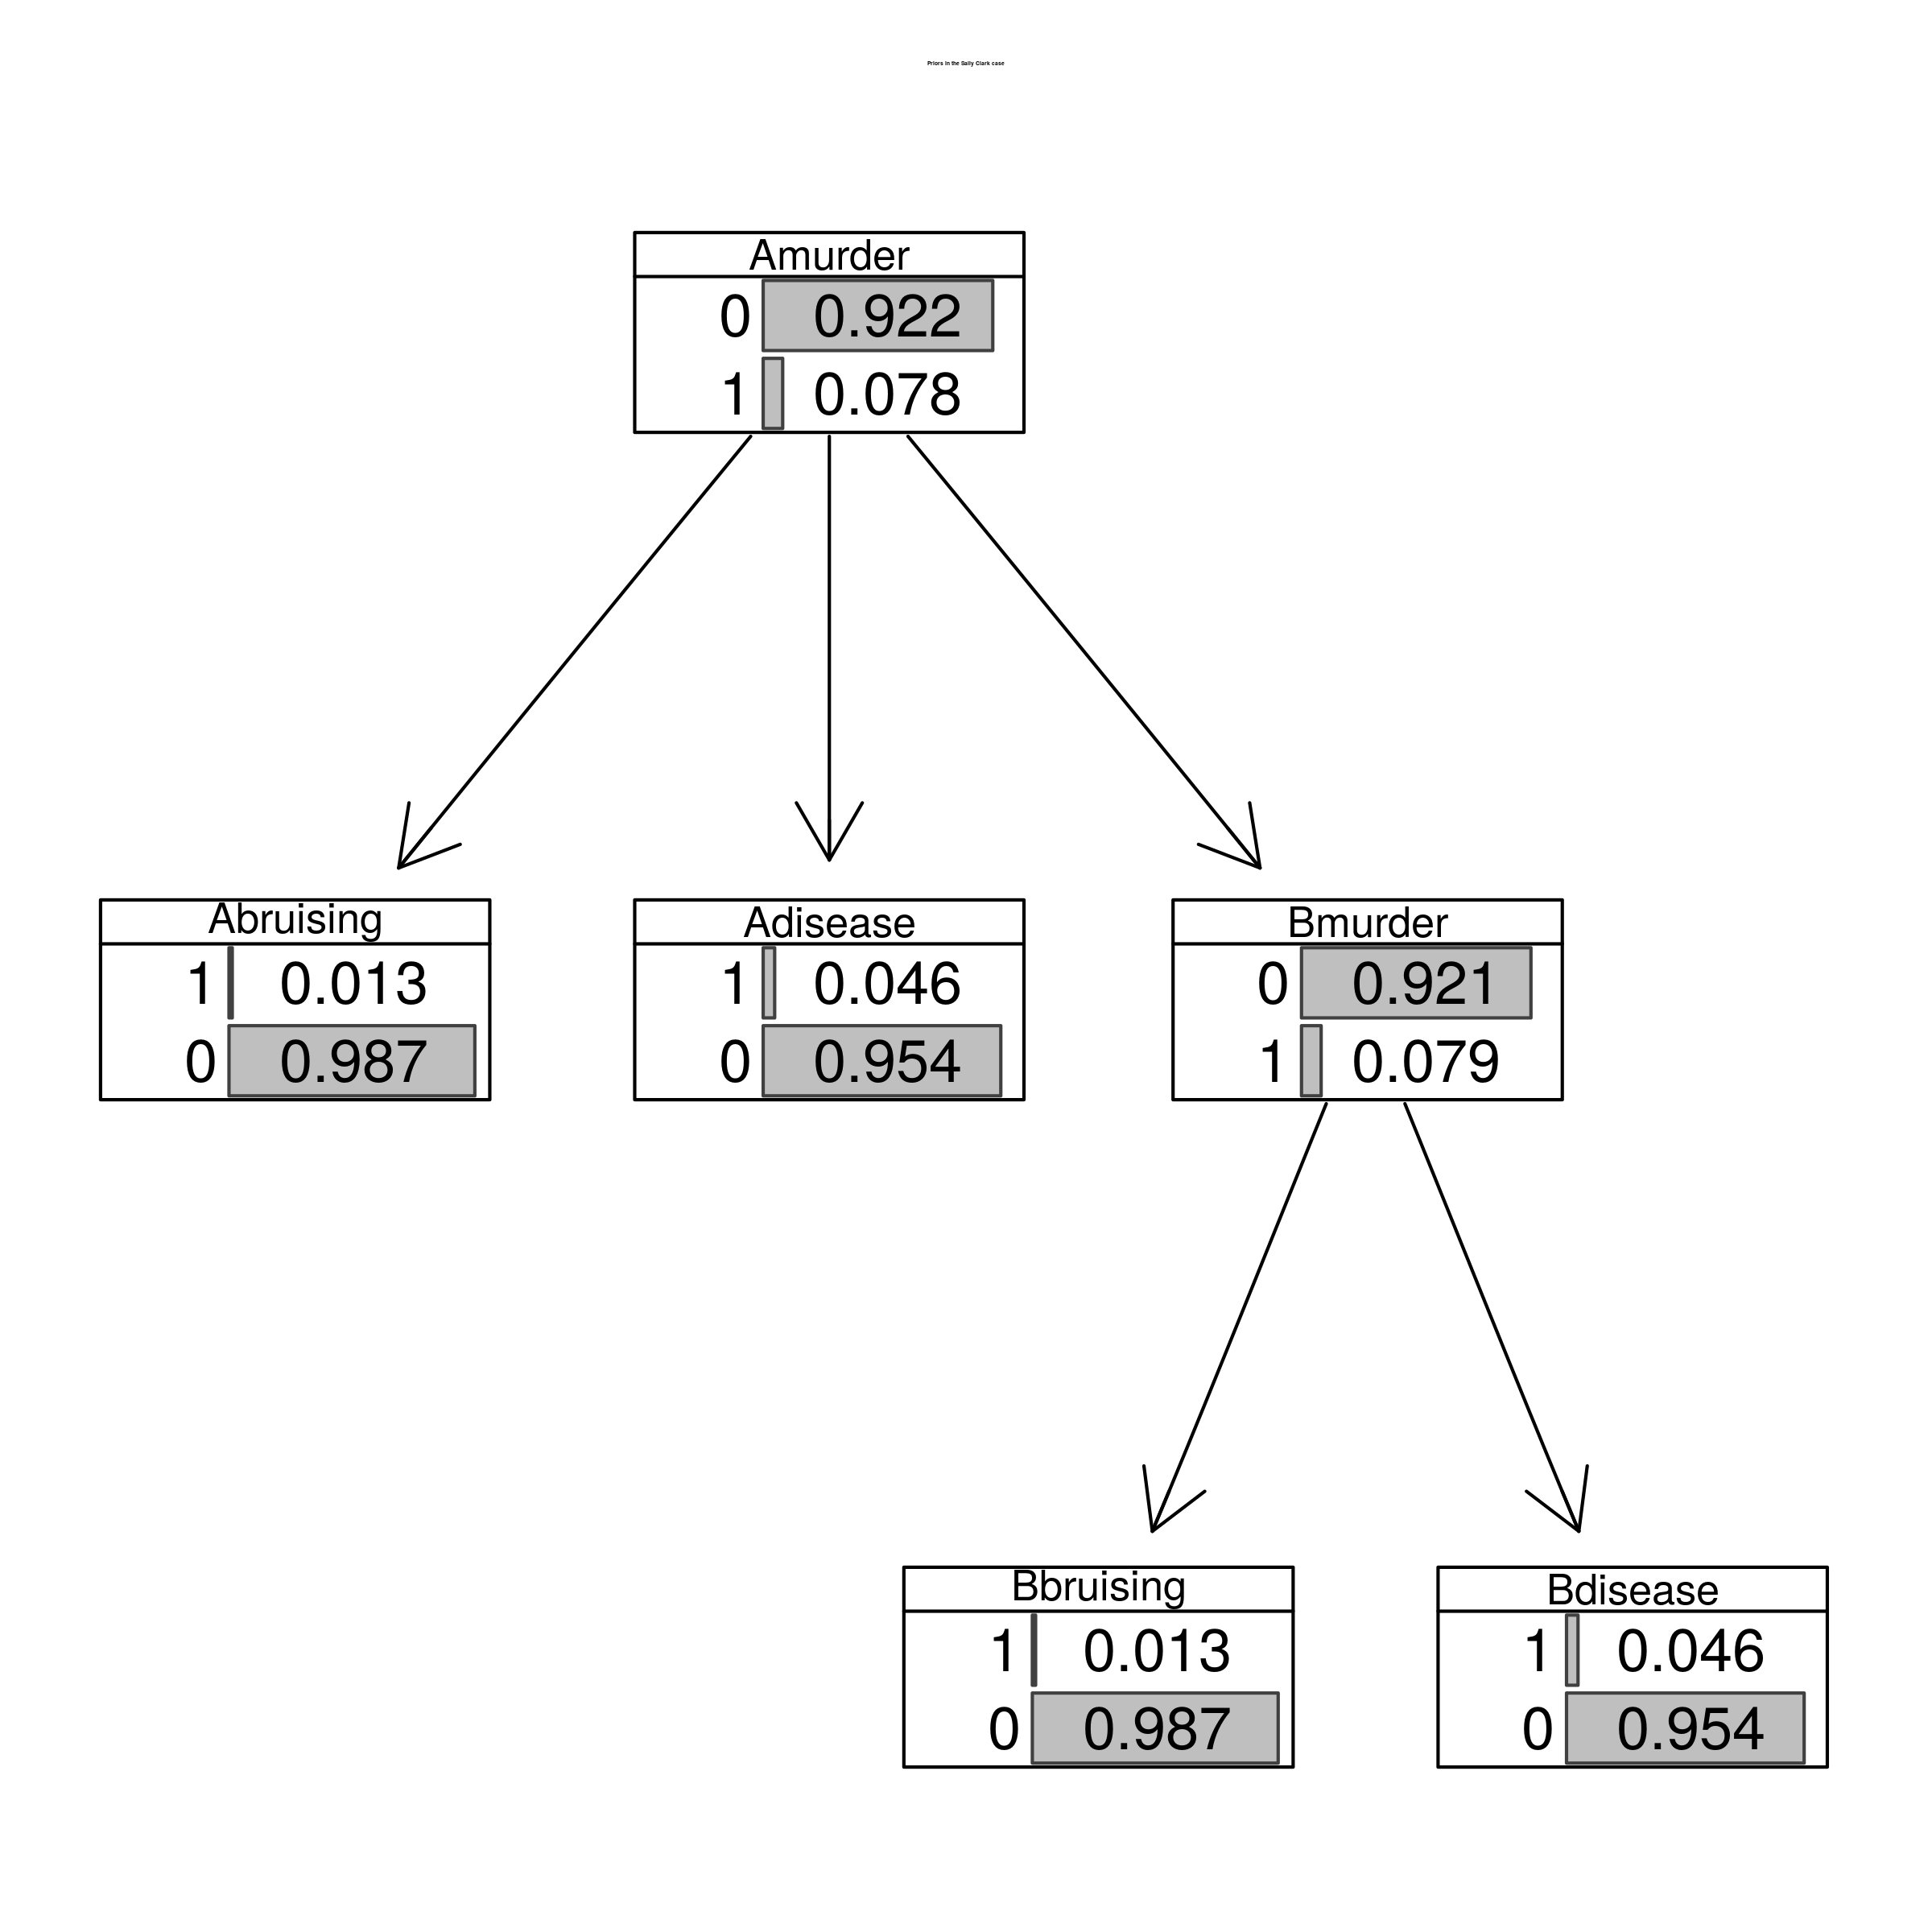
\includegraphics{SCBN.png}
    \caption{Marginal probabilities for the Sally Clark network}
    \label{fig:SCBN}
\end{figure}










\begin{figure}[h]
\hspace{10mm}
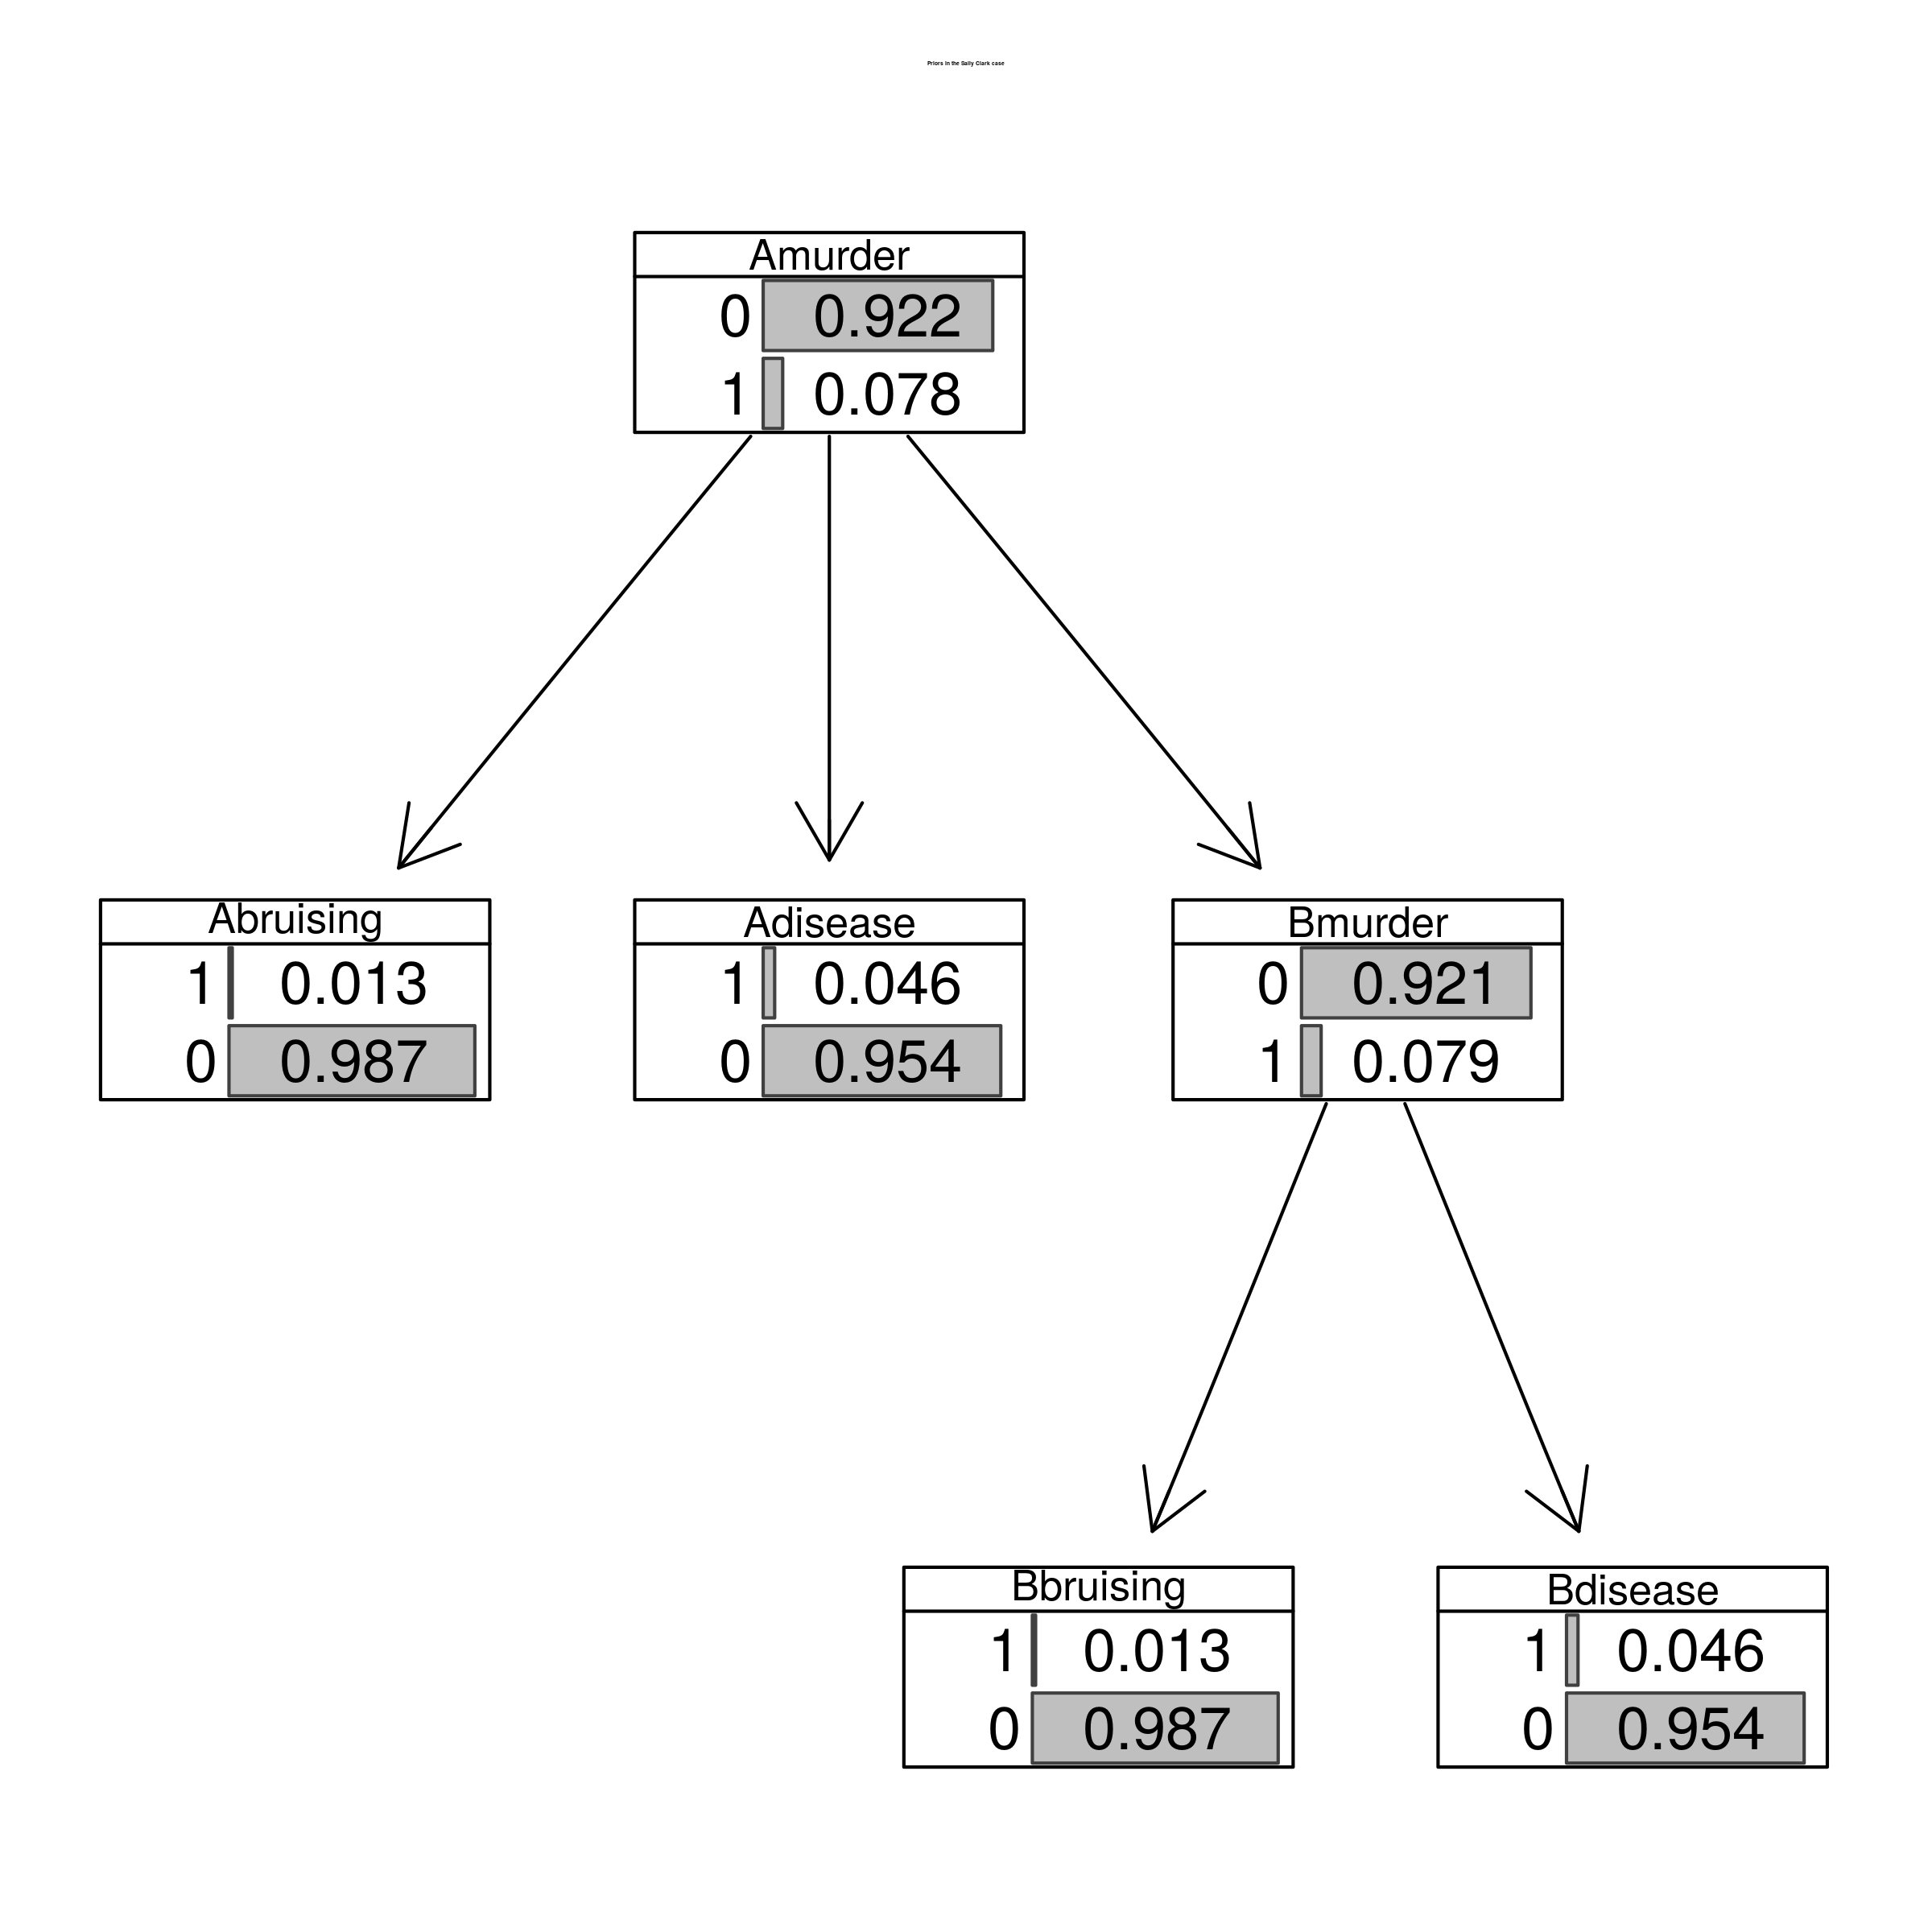
\includegraphics[width =12cm]{SCBN.png}
\caption{Bayesian network for the Sally Clark case, with marginal probabilities.}
\label{fig:BeatlesBN}
\end{figure}





\section{Challenges and ways out}\label{sec:challenges}


The known challenges to the existing measures  consist in discrepancies with intuitions in various thought experiments \citep{Merricks1995,shogenji1999conducive, Akiba2000Shogenjis, Shogenji2001Reply, bovens2004bayesian,Siebel2004On-Fitelsons-me,siebel2006against,Shogenji2006Why,crupi2007BayesianMeasuresEvidential, koscholke2016evaluating, Schippers2019General}. We try a more principled approach,  making a few more general conceptual points that suggest a way forward. 
















\subsection{Mean}\label{sec:mean}

% While the challenges have been discussed separately, considering some of them jointly also leads to an insight. Only one counterexample,
One thing to observe is that \textsf{The Beatles} is a logically inconsistent scenario. However, each  measure considered so far gives it a higher score than to multiple  logically consistent scenarios, such as \textsf{W3}\& \textsf{W4} in  \textsf{The Witnesses}. This  disagrees with our fundamental
intuition that a coherence measure should keep track of logical
consistency. 



\begin{table}
\centering
\begin{tabular}{lrrr}
\toprule
  & Fitelson & Douven-Meijs & Roche\\
\midrule
\cellcolor{gray!6}{Witness W3W4 (11)} & \cellcolor{gray!6}{-0.2336} & \cellcolor{gray!6}{-0.1103} & \cellcolor{gray!6}{0.3147}\\
Beatles (11111) & -0.0361 & 0.0247 & 0.3222\\
\bottomrule
\end{tabular}
\caption{Three coherence measures applied to a consistent  (Witness, variant W3W4) and an inconsistent scenario (Beatles).}
\end{table}

Our hypothesis is that the cause of this issue is as follows. Each measure that faces this problem  uses subsets of a set (or pairs thereof) and then takes the average
result calculated for these subsets or pairs of subsets. However, simply
taking the mean of results so obtained might be misleading, because a
few low values (for the inconsistent subsets), which indicate
inconsistency, might be mixed with many positive values (especially if a
set is large), and taking the mean of all such results might give a
relatively high score, despite involving an inconsistency. Therefore, we
believe that a candidate for a coherence measure shouldn't simply take
mean mutual confirmation scores.

\subsection{Structure}

In the existing discussion, each scenario was represented as a set of
propositions. However, it seems that usually we do not face sets of
propositions but rather scenarios with some more or less explicit
narration, which also indicates how the propositions are supposed to be
connected. In other words, agents not only report their object-level
beliefs, but also have some idea about their structure: which are
supposed to support which. This relation rarely is universal in the
powerset of the scenario (minus the empty set of course), and so
considering support between all possible pairs of propositions in the
scenario in calculating coherence might be unfair towards the agent. We
penalize her for lack of support even between those propositions which
she never thought supported each other.

To notice that the selection and direction of support arrows matter, 
consider two agents whose claims are as follows:\footnote{This example is inspired by a scenario discussed in \citep[50]{bovens2004bayesian} and \citep{Meijs2007Alleged}.}

\vspace{2mm}

\begin{center}
\begin{tabular}{lp{9cm}}
\textsf{Agent 1}     & Tweety is a bird, more specifically a penguin. Because it’s a penguin, it doesn’t fly.  \\
\textsf{Agent 2}     &  Tweety is a bird, and because it’s a bird, it doesn't fly. Therefore Tweety is a penguin. \\
\end{tabular}
\end{center}

\vspace{2mm}

\noindent Even though both of them involve the same atomic propositions,
the first narration makes much more sense, and it seems definitely more
coherent. It is also quite clear that the difference between narrations
lies in the explicitly stated direction of support. The approaches to
coherence developed so far do not account for this difference.

Moreover, it seems that when we present challenges and our intuitions
about the desiderata, we implicitly assume the narration involved is the
one that best fits with our background knowledge (so, Agent 1 rather
Agent 2 in the case of penguins). However, coherence measures developed
so far do not make such a fine-grained distinction between narrations,
and so the scenario which states that \textit{Tweety is BGP} (bird,
grounded, penguin) gets a lower score because, quite obviously, being a
bird disconfirms being a grounded animal. In such a calculation it
doesn't matter that no one even suggested this causal relationship. To
illustrate this intuition, think about a picture puzzle. Just because a
piece from the top right corner doesn't match a piece from the bottom
left corner, it doesn't necessarily decrease the coherence of a complete
picture. It just means you shouldn't evaluate how well the puzzle is
prepared by putting these two pieces next to each other.

We believe that only those directions of support which are indicated by
the reporting agent, or by background knowledge, should be taken into
account when measuring coherence.


\section{Structured coherence}\label{sec:structured}


Based on these observations we developed our own measure, which we call
\textit{structured coherence}. In this section we will describe how we
manage to avoid the above mentioned problems.  


In our calculations we use the \s{Z} confirmation measure \citep[see][for a detailed study and defense]{crupi2007BayesianMeasuresEvidential}. It results from a
normalization of many other measures (in the sense that whichever
confirmation measure you start with, after appropriate normalization you
end up with \s{Z}) and has nice mathematical properties, such as ranging
over \([-1,1]\) and preservation of logical entailment and exclusion. It
is defined for hypothesis \(H\) and evidence \(E\) as follows:\footnote{Of course, it might be interesting to see what would happen
with the coherence calculations if other confirmation measures are
plugged in, but this is beyond the scope of this paper.}
\begin{align*}
   \mathsf{prior} & = \pr(H) \\
   \mathsf{posterior} & = \pr(H \vert E)\\
   \mathsf{d} & = \mathsf{posterior} - \mathsf{prior} \\
       Z(\mathsf{posterior,prior}) & =  \begin{cases}
       0 & \text{if } \mathsf{prior} = \mathsf{posterior}\\
       \mathsf{d}/(1-\mathsf{prior}) & \text{if } \mathsf{posterior} > \mathsf{prior} \\
         \mathsf{d}/\mathsf{prior} & \text{o/w} 
       \end{cases}
   \end{align*}



 The running example employs the BN we
constructed for the first scenario in the \textsf{Witness} problem for \textsf{W1} \& \textsf{W2}.











Now, a very general picture of how the calculations of structured coherence  goes:

\begin{itemize}
    \item Build a Bayesian network representing the scenario.
    \item For each child node which represents an element of the scenario, calculate the expected support it gets from its parent(s). 
    \item Aggregate such expected support scores.
\end{itemize}


So say we have a Bayesian Network. How do we calculate the expected support? For any state \(s\) of
a child node \(C\) included in a narration, we are interested in the
support provided to \(C=s\) by the combinations
\(\mathsf{pa}_1, \cdots, \mathsf{pa}_n\) of possible states of its
parents. We ignore \(\mathsf{pa}_i\) excluded by the narration (so, usually, if parents belong to narration as well, there is only one state to consider). For any
remaining combination \(\mathsf{pa}_r\), the pair
\(\la C=s, \mathsf{pa}_r\ra\) is assigned  $Z$ score, where the prior is $\pr(C=s)$, and the posterior is $\pr(C=s \vert \mathsf{pa}_r)$.

In our running example, two child nodes, \textsf{W1} and
\textsf{W2} correspond to the two testimonies and these are the parented narration nodes.
 The root node, \textsf{D},
 represents the agent's initial uncertainty about who
committed the deed (the prior distribution is uniform) and is not
instantiated. 
For each parented node,  we list all combinations  of its states and the states of its parents not excluded by the narration. We do it for \textsf{W1} in the first two columns of Table 1.


\begin{table}
\begin{table}[H]
\centering
\resizebox{\linewidth}{!}{
\begin{tabular}{llrrrrrr}
\toprule
W1 & D & priorC & post &  priorN &  weightN & Z &  nZ\\
\midrule
\cellcolor{gray!6}{1} & \cellcolor{gray!6}{Steve} & \cellcolor{gray!6}{0.175} & \cellcolor{gray!6}{0.80} &  \cellcolor{gray!6}{0.981} &  \cellcolor{gray!6}{0.981} & \cellcolor{gray!6}{0.758} &  \cellcolor{gray!6}{0.743}\\
1 & Martin & 0.175 & 0.05 &  0.004 & 0.004 & -0.714 &  -0.003\\
\cellcolor{gray!6}{1} & \cellcolor{gray!6}{David} & \cellcolor{gray!6}{0.175} & \cellcolor{gray!6}{0.05} &  \cellcolor{gray!6}{0.004} &  \cellcolor{gray!6}{0.004} & \cellcolor{gray!6}{-0.714} &  \cellcolor{gray!6}{-0.003}\\
1 & John & 0.175 & 0.05 &  0.004 &  0.004 & -0.714 &  -0.003\\
\cellcolor{gray!6}{1} & \cellcolor{gray!6}{James} & \cellcolor{gray!6}{0.175} & \cellcolor{gray!6}{0.05} &  \cellcolor{gray!6}{0.004} &  \cellcolor{gray!6}{0.004} & \cellcolor{gray!6}{-0.714} &  \cellcolor{gray!6}{-0.003}\\
1 & Peter & 0.175 & 0.05 &  0.004 & 0.004 & -0.714 &  -0.003\\
\bottomrule
\end{tabular}}
\end{table}
\caption{ECS calculation table for \s{W1} in the first scenario in the \s{Witness} problem.}
\label{t:w1}
\end{table}


 We only consider cases in which \textsf{W1} holds, so we have 1s everywhere in the first column. However, the agent is not supposed to know who committed the deed, so all possible instantiations of \textsf{D} are listed.   In our example the prior probability of \s{W1} is in column \textsf{priorC} (prior for the \textbf{child}, it does not depend on the state of $D$, so it is constant, repeated to facilitate row-wise calculations), and the posterior probability of \textsf{W1} given different states of \textsf{D} is in column \s{post}.  We then  use these values to calculate the \s{Z} confirmation measures. In our example, these values are in column \s{Z}. 
 
 
 Now, to get from multiple \s{Z} scores to expected support levels we weight these scores by normalized  marginal probabilities of \(\mathsf{pa}_r\) \emph{as perceived from the perspective of the narration}. 
 
 \begin{align*}
    \mathsf{weightN}_i & = \frac{\mathsf{priorN}_i}{\sum \mathsf{priorN}_j}\\
    \mathsf{nZ}_{i} & = \mathsf{weightN}_i \times \mathsf{Z}_i
 \end{align*}
 
 
 \noindent (In  the cases in which the parents also belong to a narration,  each child has a single \s{Z} score.) 

 




 In our example (Table \ref{t:w1}), \textsf{priorN} gives the distribution of \textsf{D} that we would obtain if we updated the BN with \textsf{W1} = \textsf{W2} = 1, that is, with the narration in question.  \textsf{weightN} is the result of normalizing \textsf{priorN} (in this case, the probabilities already add up to 1, so this move don't change anything). Now, weight the Z score by the normalized probability, and sum these weighted Z scores, obtaining what we call the \emph{Expected Connection Strength} of the parented node under consideration.   In our example, the last column weights \textsf{Z} using  \textsf{weightN}. The \textsf{ECS} for \textsf{W1} is the sum of \textsf{nZ}, $0.728$.



 As the result of applying this procedure to all  nodes that belong to a narration, we get a list of \textit{expected connection strengths}. What do we do with the list of \textsf{ECS} scores thus obtained? For
the reasons already discussed, we don't want to simply take the mean.\footnote{The problem is a particular case of a common problem in statistics: how
to represent a set of different values in a simple way without
distorting the information too much? One easy and accurate solution is
to plot all values. The problem is, it gives us no unambiguous way to
compare different sets. For such tasks, a single score is desirable.} We
should pay special attention to \s{mean}  and \s{minimum}. The
mean gives us an idea of how strong the average support between the
elements is.\footnote{This might seem  in line with the average mutual support
measures. However, on our approach we only care about specific directions of support.}  We also look at the minimum, because special attention should be paid to weaker links: the
weaker such links are, the less trust should be placed in a narration.
The presence of strong links doesn't have to make up for the impact of weak
links --- after all, adding information to a fairly incoherent scenario shouldn't increase its coherence much.\footnote{To
take the simplest example, if two elements are logically inconsistent, the whole narration is incoherent, even if some of its other elements cohere to a large degree. Imagine two narrations. In the first one, you have a case where all
parent-child links except one get the maximal positive score. The
remaining one gets the score of -1. We submit that the overall score
should be -1. In the second narration all the relations take a value
close to -1. We share the intuition that the narration still should have
a higher overall score than -1. The presence of an element with the
posterior that equals 0 (which is needed for \(Z\) confirmation being
-1) means that the probability of the whole scenario itself is null, which is clearly lower than whatever low posterior the other scenario might have.}






So here's our stab at a mathematical explication of a coherence measure
that satisfies the desiderata we just discussed. We are not deeply
attached to its particularities and clearly other ways of achieving this
goal may we worth pursuing.

\begin{itemize}
\item  If all values are non-negative, i.e. each relation between parents and a child is supportive, then even the weakest point of a story is high enough not to care about it. In such cases we take $\s{mean}$ as the final result.

\item If, however, some values are negative, we need to be more careful. We still look at  $\s{mean}$, but  the lower the minimum, the less attention we should pay to it, and the more attention we should pay to the minimum. If the minimum is -1, we want to give it full weight, $1 = \vert \s{min}\vert = - \s{min}$ and ignore (weight by 0) $\s{mean}$. In general, we propose to use $\vert \s{min}\vert$  as the weight assigned to the minimum, and  $1-\vert \s{min}\vert$  to weight $\s{mean}$.  For instance, if the minimum is -0.8, the weight of  $\s{mean}$ should be $-0.8+1 = 0.2$, while if it is $-0.2$, this weight is $0.8$.\footnote{Again, there are other ways to mathematically capture the intuition that the lower minimum, the more attention is to be paid to it, but we decided to take the most straightforward way of doing so for a ride.}  Note that  $1-\vert \s{min}\vert =  1-\vert \s{min}\vert = 1 - (- \s{min}) = 1+\s{min}$, and so the  formula is:
\end{itemize}

Thus, the full formula is as follows:

\footnotesize

\begin{align*}
\mathsf{Structured}(\mathsf{ECS}) & = \begin{cases}
\mathsf{mean}(\mathsf{ECS})  \times \left(\textsf{min}(\mathsf{ECS})+1 \right) - \textsf{min}(\mathsf{ECS})^2   & \text{if } min(\mathsf{ECS})<0 \\\mathsf{mean}(\mathsf{ECS}) & \text{o/w}
\end{cases}
\end{align*}

\normalsize





This function has a desired property which was missing in most of the
other coherence measures. Whenever we encounter a logically inconsistent
story, i.e.~a story with the lowest possible minimum (in our measure it
is -1), we'll end up with -1 also as the final score. The achieved
results are also plausible if the minimum is close to the lowest
possible value.



Thus, our coherence measure is be a function of a series of expected  confirmation scores. This is somewhat in line with average mutual
support measures which took the coherence of a set to be a function of
confirmation scores. One key difference, however, is that average mutual
support measures used confirmation scores for all disjoint pairs of
non-empty subsets of a given set, and our measure will only rely on the
confirmation scores for the support relations indicated by the BN
representing a narration. This is because we don't think a narration
should be punished for the lack of confirmation between elements that
were never intended to be related. Another difference is that while average mutual support measure take simply confirmation levels, we take them as expected from the perspective of a given narration.






% Now, let's take this coherence measure for a ride.

\subsection{Updated weights?}



We think that what this example illustrates is that we should really
carefully think about whose cognitive perspective is taken when we
represent a narration using a BN, focusing on whether the BN involves
nodes which are not part of the narration whose coherence is to be
evaluated. In particular, the probabilistic information about the
uniform distribution of guilt probability is not part of any of the
three involved narrations, but rather a part of a third-person set-up
prior to obtaining any evidence.

To evaluate the coherence of a narration, at least for unmentioned
assumptions that one doesn't have strong independent reasons to keep,
one should think counterfactually, granting the consequences of the
narration and asking what would happen if it indeed was true. 



In our
case, a judge who evaluates the coherence of witness testimonies once
she has heard them, no longer thinks that the distribution of \textsf{D}
is uniform. And this agrees with the counterfactual strategy we just
described: it is a consequence of the probabilistic set-up and the
content of \textsf{W1} and \textsf{W2} that if \textsf{W1} and
\textsf{W2} were true, the distribution for \textsf{D} no longer would
be uniform, and so it is unfair to judge the coherence of this scenario
without giving up this assumption and updating one's assumptions about
\textsf{D}.

In such a case, we think, we should update \textsf{D} to what it would
be had \textsf{W1} and \textsf{W2} be instantiated with 1s:

\begin{table}[H]
\centering
\begin{tabular}{lrrrrrr}
\toprule
  & Steve & Martin & David & John & James & Peter\\
\midrule
\cellcolor{gray!6}{Pr} & \cellcolor{gray!6}{0.981} & \cellcolor{gray!6}{0.004} & \cellcolor{gray!6}{0.004} & \cellcolor{gray!6}{0.004} & \cellcolor{gray!6}{0.004} & \cellcolor{gray!6}{0.004}\\
\bottomrule
\end{tabular}
\end{table}

\noindent and use these updated probabilities to build the weights used
in our coherence calculations for this narration (and proceed
accordingly, instead updating on another set of narration nodes in the
coherence evaluation of other
narrations).\footnote{Note  however that  you should not simply instantiate the BN with \textsf{W1} and \textsf{W2}, propagate and run the coherence calculations on the updated BN. Then both these nodes would get 1s in their respective CPTs and coherence calculations would make   all  confirmation measures involved in such calculations  based on posterior probability equal 1. If narration members have probability one, no other information will be able to confirm it.}
Once this strategy is taken, the problem turns out to be not that
challenging for any of the coherence measures under discussion.




\section{Coherence in Sally Clark}\label{sec:Sally}


First, we are interested in the coherences assigned to different scenarios in the Sally Clark case prior to any evidence regarding bruising or disease. Call this Stage 0. Calculations for the coherence measures mentioned in the paper are as in Table \ref{tab:SCcoherenceNoEvidence}.

\pagebreak 

\begin{table}[H]
   \resizebox{\linewidth}{!}{
\begin{tabular}[t]{lrrrrrrr}
\toprule
States & Structured & Fitelson & Douven-Meijs & Roche & Shogenji & Olsson-Glass & Probability\\
\midrule
00 & 0.1984 & 0.9924 & 0.0783 & 0.9997 & 1.0850 & 0.9993 & 0.9211\\
11 & 0.2000 & 0.9993 & 0.9176 & 0.9962 & 12.6694 & 0.9924 & 0.0783\\
01 & -0.9855 & -0.9998 & -0.4996 & 0.0001 & 0.0002 & 0.0000 & 0.0000\\
10 & -0.9997 & -0.9919 & -0.4962 & 0.0041 & 0.0081 & 0.0006 & 0.0006\\
\bottomrule
\end{tabular}}
    \caption{Coherence scores and  probabilities for the Sally Clark BN prior to evidence regarding bruising or disease.}
    \label{tab:SCcoherenceNoEvidence}
\end{table}


Compare it to Stage A, when bruising was considered found in both sons but signs of disease in none (Table \ref{tab:SCcoherenceStageA}).

\begin{table}[H]
\resizebox{\linewidth}{!}{
\begin{tabular}[t]{lrrrrrrr}
\toprule
States & Structured & Fitelson & Douven-Meijs & Roche & Shogenji & Olsson-Glass & Probability\\
\midrule
00 & 0.1990 & 0.9985 & 0.6997 & 0.9983 & 3.3430 & 0.9966 & 0.2981\\
11 & 0.2000 & 0.9966 & 0.2979 & 0.9993 & 1.4247 & 0.9985 & 0.7009\\
01 & -0.9914 & -0.9999 & -0.4995 & 0.0000 & 0.0001 & 0.0000 & 0.0000\\
10 & -0.9998 & -0.9952 & -0.4981 & 0.0024 & 0.0048 & 0.0010 & 0.0010\\
\bottomrule
\end{tabular}}
\caption{Coherence scores and  probabilities for the Sally Clark BN after evidence of bruising in both sons and of no   disease in both.}
\label{tab:SCcoherenceStageA}
\end{table}

Finally, let's also inspect the coherence scores for Stage B, in which bruising was found in both, but signs of disease were present in son A (Table \ref{tab:SCcoherenceStageB})


\begin{table}[H]
\resizebox{\linewidth}{!}{
\begin{tabular}[t]{lrrrrrrr}
\toprule
States & Structured & Fitelson & Douven-Meijs & Roche & Shogenji & Olsson-Glass & Probability\\
\midrule
00 & 0.1854 & 0.9346 & 0.0426 & 0.9983 & 1.0446 & 0.9966 & 0.9541\\
11 & 0.2000 & 0.9967 & 0.9207 & 0.9650 & 21.7984 & 0.9300 & 0.0427\\
01 & -0.8727 & -1.0000 & -0.4984 & 0.0000 & 0.0000 & 0.0000 & 0.0000\\
10 & -0.9999 & -0.9312 & -0.4649 & 0.0367 & 0.0731 & 0.0032 & 0.0032\\
\bottomrule
\end{tabular}}
\caption{Coherence scores and  probabilities for the Sally Clark BN after evidence of bruising in both sons and of   disease in son A.}
\label{tab:SCcoherenceStageB}
\end{table}


Here  are some observations with respect to what we would intuitively expect.



\begin{itemize}
    \item We would expect both 01 and 10 to have much lower coherence than 11 or 00. This condition is satisfied by all measures.
    \item  In Stage 0 we would expect the coherences of 00 and 11 to be close. This requirement fails for Douven-Meijs and Shogenji.
    \item Perhaps, we would not expect 11 and 00 to be nearly maximally coherent. If we buy into this intuiton, we have reasons to dislike Fitelson, Roche and Olsson-Glass.
    \item When moving from Stage 0 to Stage 1, the coherence of 11 should not decrease. After all, we include evidence in support of 11. This condition fails for Douven-Meijs, Shogenji and to a slight extent for Fitelson.
    \item For similar reason, we would not expect the coherence of 11 to be much less than the coherence of 00 in Stage A. This condition fails for Douven-Meijs and Shogenji.
    \item Given that in Stage B we include evidence supporting the claim that son A was not murdered, we would not expect the coherence of 01 to be smaller than the coherence of 10 in Stage B. This condition fails radically for Fitelson (01 becomes maximally incoherent, even though the evidence is not conclusive!), and to a small degree for Douven-Meijs.
\end{itemize}


Another interesting observation arises when we take all the table rows as data points and think about the truth-conduciveness of coherence. While scenarios with high coherence, presumably, can have various probabilities, we might have the intuition that coherence is at least a negative criterion: scenarios with very low coherence should tend to have low probability. What's the situation with the four scenarios in the three stages we discussed, with respect to all the measures we discussed? Well, this condition holds for all measures except for Douven-Meijs and Shogenji, where scenarios with higher coherence tend to have much lower probability than scenarios with relatively neutral coherence, which we find somewhat surprising (Figure \ref{fig:cohplot}).



\begin{figure}
    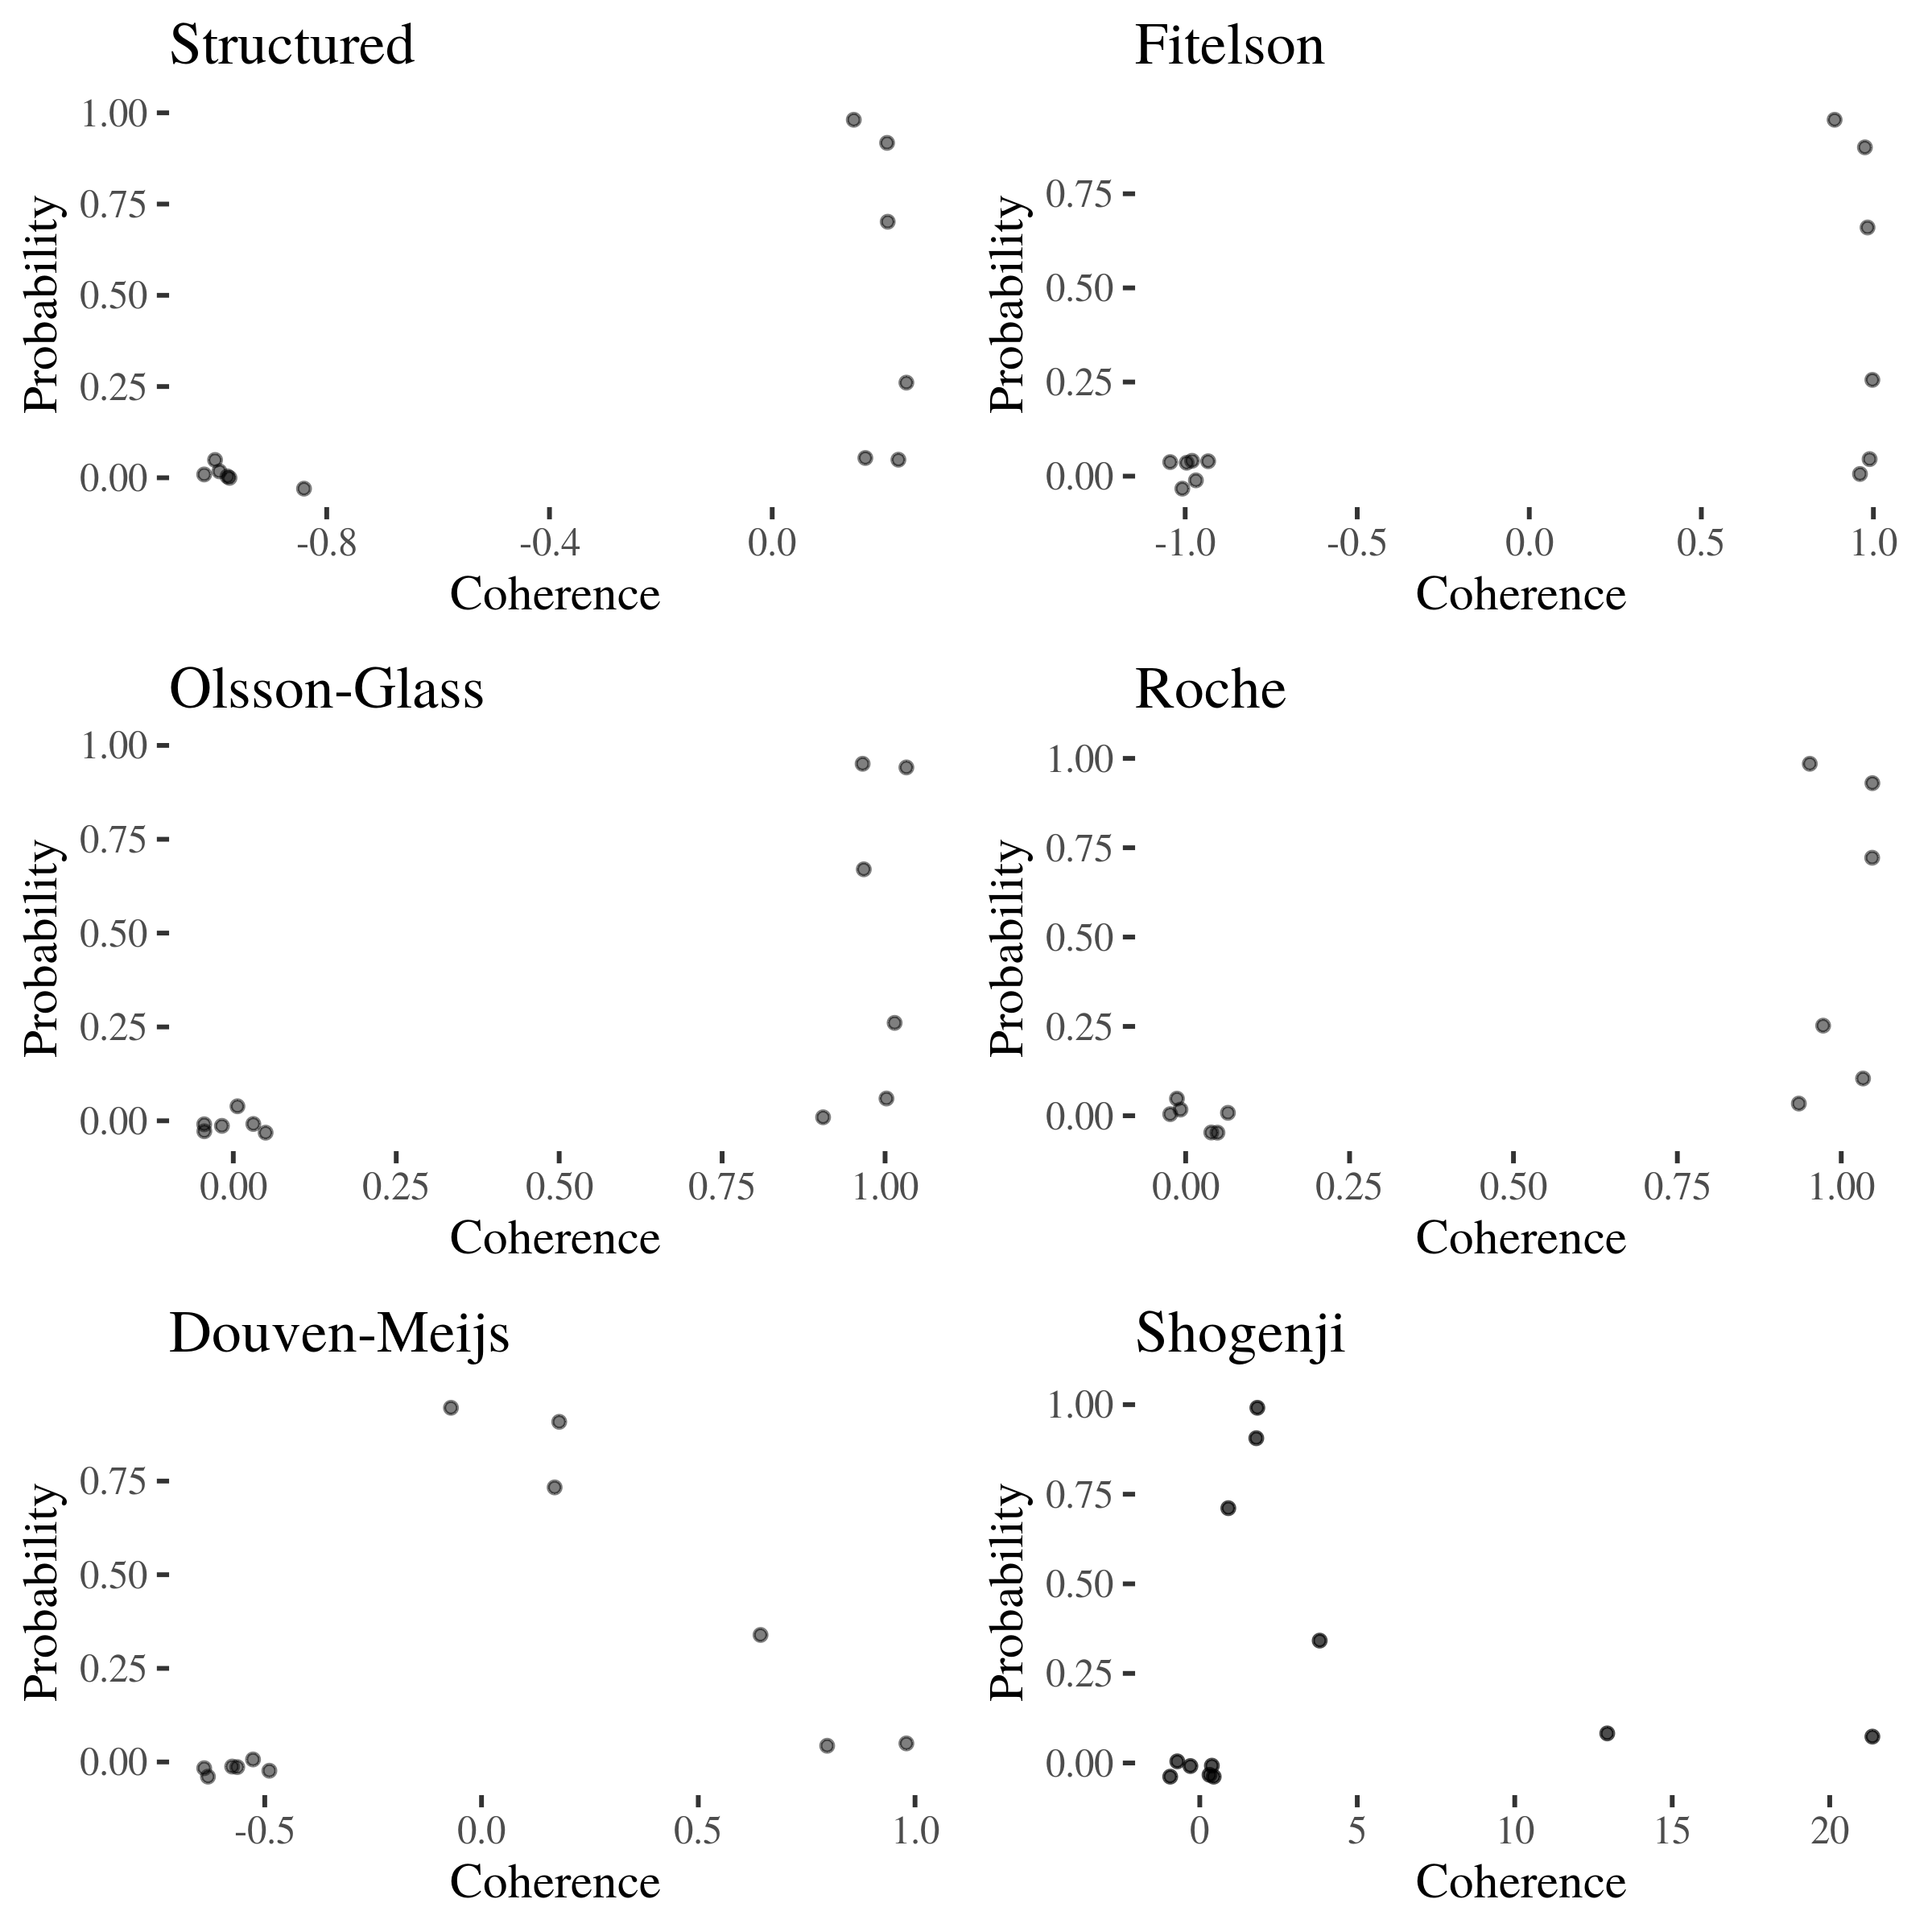
\includegraphics{cohPlots.png}
    \caption{Probability vs. coherence by coherence measure. Note the unusal patterns for Douven-Meijs and Shogenji, and agreement in patterns for the other measures.}
    \label{fig:cohplot}
\end{figure}





\section{Some results \& discussion}\label{sec:discussion}

\begin{table}[H]
    \resizebox{\linewidth}{!}{
\begin{tabular}{lrrrrrr}
\toprule
  & Structured & Fitelson & Douven-Meijs & Roche & Shogenji & Olsson-Glass\\
\midrule
\cellcolor{gray!6}{Beatles: JPGRD 11111} & \cellcolor{gray!6}{-1} & \cellcolor{gray!6}{-0.0361} & \cellcolor{gray!6}{0.0247} & \cellcolor{gray!6}{0.3222} & \cellcolor{gray!6}{0} & \cellcolor{gray!6}{0}\\
\bottomrule
\end{tabular}}    \caption{Coherence scores in the Beatles scenario.}
    \label{tab:beatles}
\end{table}




\begin{table}[H]
\resizebox{\linewidth}{!}{
\begin{tabular}{lrrrrrr}
\toprule
  & Structured & Fitelson & Douven-Meijs & Roche & Shogenji & Olsson-Glass\\
\midrule
\cellcolor{gray!6}{Witness: W1W2 11} & \cellcolor{gray!6}{0.7294} & \cellcolor{gray!6}{0.7711} & \cellcolor{gray!6}{0.4464} & \cellcolor{gray!6}{0.6214} & \cellcolor{gray!6}{3.5510} & \cellcolor{gray!6}{0.4508}\\
Witness: W3W4 11 & 0.4944 & -0.2336 & -0.1103 & 0.3147 & 0.7405 & 0.1867\\
\cellcolor{gray!6}{Witness: W4W5 11} & \cellcolor{gray!6}{0.6016} & \cellcolor{gray!6}{0.2183} & \cellcolor{gray!6}{0.1103} & \cellcolor{gray!6}{0.5353} & \cellcolor{gray!6}{1.2595} & \cellcolor{gray!6}{0.3655}\\
\bottomrule
\end{tabular}}    \caption{Coherence scores for the witness scenarios.}
    \label{tab:witnesses}
\end{table}














In light of conceptual problems with the existing coherence measures we have developed a Bayesian-network based coherence measure that relies not only on the probability measure, but also on the underlying network structure. 

One question is whether it handles the philosophical counterexamples present in the literature. The answer is, it does, but these issues will be covered in a different paper, as this discussion is quite extensive. 

A potential, more practice-oriented  application of this tool is to investigate coherence in  Bayesian networks based on real-life legal cases--- our treatment of the Sally Clark case is only a small step in this direction. This remains a project for the future.

Another line of investigation concerns
the potential use of coherence to    estimate model priors for Bayesian model averaging, which might be useful in legal contexts might be more fair  than using equal or fixed priors or unprincipled intuitive assessment of priors. 




























\bibliographystyle{apalike}

\bibliography{coherence}

\end{document}